%%%%%%%%%%%%%%%%%%%%%%%%%%%%%%%%%%%%%%%%%%%%%%%%%%%%%%%%%%%%%%%%%%%
%
% IMPERIAL COLLEGE LONDON DISSERTATION TEMPLATE 
%
%%%%%%%%%%%%%%%%%%%%%%%%%%%%%%%%%%%%%%%%%%%%%%%%%%%%%%%%%%%%%%%%%%%
%
% Copyright (c) 2008, Daniel Wagner, www.PrettyPrinting.net
% http://www.prettyprinting.net/imperial/
%%%%%%%%%%%%%%%%%%%%%%%%%%%%%%%%%%%%%%%%%%%%%%%%%%%%%%%%%%%%%%%%%%%

\documentclass[MSc,paper=a4,pagesize=auto]{icldt}
%\usepackage{showframe}
%\usepackage{cleveref} % lets us use chapter references
\usepackage{graphicx}  % lets us import graphics nicely
\usepackage{caption}   % to go with lstlisting
\usepackage{subcaption}  % lets us use subfigure
\usepackage[binary-units=true]{siunitx}   % and friendly SI unit shiz
\setcounter{tocdepth}{1} % don't show sub-sections in the TOC
% next two lines supress 'underfull hbox" warnings caused by URLs in bib file
\usepackage{etoolbox}
\apptocmd{\sloppy}{\hbadness 10000\relax}{}{} 
\usepackage{todonotes}  % TODO
\usepackage{dirtree}    % directory structure

\usepackage{scrhack}  % to avoid the warning that \float@addtolists is deprecated
\usepackage{listings} % lets us insert software code and highlight
\usepackage{color}    % required to set background colour
\lstset{
	language=[Visual]C++,
	keywordstyle=\bfseries\ttfamily\color[rgb]{0,0,1},
	identifierstyle=\ttfamily,
	commentstyle=\color[rgb]{0.133,0.545,0.133},
	stringstyle=\ttfamily\color[rgb]{0.627,0.126,0.941},
	showstringspaces=false,
	basicstyle=\tiny, %small,
%	numberstyle=\footnotesize,
%	numbers=left,
%	stepnumber=1,
%	numbersep=5pt,
	tabsize=2,
	breaklines=true,
	prebreak = \raisebox{0ex}[0ex][0ex]{\ensuremath{\hookleftarrow}},
	breakatwhitespace=true,
	aboveskip={1.5\baselineskip},
%	captionpos=b,
  columns=fixed,
  extendedchars=true,
  backgroundcolor=\color[rgb]{0.9,0.9,0.9},%\color{white},
%  title=\lstname
}

%\usepackage[usenames,dvipsnames]{color} % know about colours
\definecolor{grey}{RGB}{102,102,102}
\DeclareCaptionFont{white}{\color{white}}
\DeclareCaptionFormat{listing}{\colorbox{grey}{\parbox{0.97\textwidth}{#1#2#3}}}
\captionsetup[lstlisting]{format=listing,labelfont=white,textfont=white}

% Questionairre definitions based on Sven Hartenstein's examples
%%%%%%%%%%%%%%%%%%%%%%%%%%%%%%%%%%%%%%%%%%%%%%%%%%%%%%%%%%%%%%%%%%%%%%
\usepackage{wasysym}% provides \ocircle and \Box
\usepackage{enumitem}% easy control of topsep and leftmargin for lists
\usepackage{forloop}% used for \Qrating and \Qlines
\usepackage{ifthen}% used for \Qitem and \QItem
\usepackage{typearea}

\newcommand{\Qq}[1]{\textbf{#1}}
\newcommand{\QO}{$\Box$}% or: $\ocircle$
\newcounter{qr}
\newcommand{\Qrating}[1]{\QO\forloop{qr}{1}{\value{qr} < #1}{---\QO}}
\newcommand{\Qline}[1]{\noindent\rule{#1}{0.6pt}}
\newcounter{ql}
\newcommand{\Qlines}[1]{\forloop{ql}{0}{\value{ql}<#1}{\vskip0em\Qline{\linewidth}}}
\newenvironment{Qlist}{%

\renewcommand{\labelitemi}{\QO}
	\begin{itemize}[leftmargin=1.5em,topsep=-.5em]}{ \end{itemize} 
}	
\newlength{\qt}
\newcommand{\Qtab}[2]{
	\setlength{\qt}{\linewidth}
	\addtolength{\qt}{-#1}
	\hfill\parbox[t]{\qt}{\raggedright #2}
}
\newcounter{itemnummer}
\newcommand{\Qitem}[2][]{% #1 optional, #2 notwendig
	\ifthenelse{\equal{#1}{}}{\stepcounter{itemnummer}}{}
	\ifthenelse{\equal{#1}{a}}{\stepcounter{itemnummer}}{}
	\begin{enumerate}[topsep=2pt,leftmargin=2.8em]
	\item[\textbf{\arabic{itemnummer}#1.}] #2
	\end{enumerate}
}
%%%%%%%%%%%%%%%%%%%%%%%%%%%%%%%%%%%%%%%%%%%%%%%%%%%%%%%%%%%%%%%%%%%%

% Essential Setup
\title{Seeing the Big Data: Virtual Reality Visualisations of Large Datasets}
\author{Alexander Zawadzki (az2713)}
\date{September 2014}
\department{Computing}

% Optional
\supervisor{Professor Daniel Rueckert} 
\dedication{
My thanks to: 
\newline
\newline
Dr Paul Gass and Dr Ian Thompson, my bosses at Sharp Laboratories of Europe Ltd., for arranging for my funded sabbatical year at Imperial College London. 
\newline
\newline
Colleagues 	Dr Nathan Smith, Dr Graham Jones, Dr Jon Mather, and Dr Andrew Kay for sharing their passion for 3D display systems. Especial thanks to John Nonweiler, for setting an example of how development software \textit{should} be done.
\newline
\newline
Supporters Aashish Chaudhary at Kitware, and Brad Davis at ORIA for providing insight into VTK and the Oculus Rift SDK respectively.
\newline\
\newline
Friends in the MCS Program, in particular coffee-break-buddies Moritz Schrenk and Tereza Drskova. 
\newline
\newline
And last, but not least, I am indebted to my supervisors Professor Daniel Ruckert and Dr Bernhard Kainz. You have provided freedom when I wanted it, and guidance when I needed it. I am deeply grateful to you both. 
}

\begin{document}
\maketitle

\begin{abstract}
%\textbf{A Zawadzki, Department of Computing, Imperial College London}
%\\ \textbf{Abstract of Master's Thesis, submitted September 4th 2014}
%\\ \textbf{Seeing the Big Data: Virtual Reality Visualisations of Large Datasets}
A new pipeline is implemented for the visualisation of Human Connectome Project (HCP) data. HCP data are converted to an intermediate format, and then imported into the Visualisation Tool Kit (VTK). Through a series of extensions to the VTK pipeline, the data are rendered as distorted stereographic 3D images and output to an Oculus Rift virtual reality headset. Sensors on the headset track the user's head position and dynamically update the rendered image. The complete pipeline allows an immersive 3D display of data, with native access to all VTK functionality. A user study is conducted to evaluate the pipeline, and the strengths and weaknesses are discussed.

%\hfill --- Alexander Zawadzki

\end{abstract}

\makededication
%\iffalse
\tableofcontents

\listoftables
\listoffigures


\chapter{Introduction}
\section{Context}
In order to better understand the functioning of the human brain, the neurology of the brain is very important. The ongoing Human Connectome Project (in the USA) and the Developing Human Connectome Project (in the UK) are dedicated to mapping and analysing the neural connections of developed and developing human brains. 

These Connectome projects produce very large datasets giving information about the structural and functional connectivity of neurons in the brain. Multi-gigabyte datasets are common, as of June 2014 the Human Connectome Project has generated over 20 terrabytes of data. The volume of data produced, and 3D nature of the data can make it difficult to visualise in 2D form. A typical functional connectome matrix, for example, may have 3,000 by 3,000 elements and in 2D form bears no resemblance to the physical shape of the fibres.

Advances in computing power and display technology offer the capability to visualise these data sets in new ways. The dominant display technology today is the LCD computer monitor: large, high resolution, but a 2D format. Recent developments in virtual reality technology, in particular the mass-market launch of Oculus Rift development kits, offer new and exciting opportunities.

But, do researchers want to view data in 3D? What data is suited to this type of display? Is the performance of current VR display systems good for practical purposes? This project has sought to answer these questions by developing a demonstration system for the virtual reality display of medical image data. The demonstration system was used to conduct a survey in the Biomedical Image Analysis Group, and gather expert feedback. Results showed a significant interest in the use of Virtual Reality visualisation tools, and suggestions provided many ideas for further development.

\newpage
\section{Contributions}
This project has investigated the use of consumer grade virtual reality hardware, specifically the Oculus Rift DK1, as a tool for visualising and interacting with large datasets. The project has contributed to the open source community in a number of ways:

\begin{itemize}
  \item Source code was ported from Paraview with encouragement from lead developer Aashish Chaudhary in order to bring Rift functionality to VTK.
  \item A plug-in was developed for Blender in order to allow the import of legacy\footnote{Although technically a 'legacy' format, plain text vtk files are as widely used as their 'modern' XML format counterparts.} .vtk format data.
  \item A number of bugs were identified and fixed in the Linux version of the excellent Oculus Rift in Action (ORIA) project. The project was forked on GitHub, at the suggestion of the project owner Brad Davis, to share these bug-fixes with the community.
  \item When relevant, assorted software problems were documented on Stack Overflow in 'Question and Answer' format. The response to these posts has been very positive, bumping my account "\textit{GnomeDePlume}" to the top quartile of contributors in 2014.  
\end{itemize}

In comparison to the size and scope of the VTK, Blender and ORIA projects, the contributions to these projects have been very small. Nevertheless, contributions were made in the spirit of open source collaboration and have have incrementally advanced the state-of-the-art.

The academic impact of this work has been modest: numerous demonstrations within the Biomedical Image Analysis Group, and a formal presented to my employers at Sharp Laboratories of Europe\footnote{Following which they offered me a raise, so some good has come of it.}. Although this MCS thesis will be the main academic publication resulting from the project, it is hoped that the documented source code, image content and demonstration system will be a useful resource for future project work.

\newpage
\section{Structure of the Report} 
\label{sec:structure_of_the_report}
As the project dealt with implementing a pipeline, illustrated in Figure~\ref{fig:the_full_pipeline}, it seems natural for the report to follow the process from raw data acquisition to the final display image. 

Following this logic, Chapter~2 discusses the how the Human Connectome Project (HCP) maps human brain structures using DTI and fMRI imaging, and discusses existing visualisation techniques. Chapter~3 discusses the HCP data structure, and how it may be converted to intermediate formats. Chapter~4 shows how a Visualisation Tool Kit (VTK) pipeline can be constructed and HCP data can be processed for interaction and display on a standard 2D computer monitor. 

Chapter~5 breaks away from the sequential structure in order to introduce the Oculus Rift hardware, and shows how the collimating optics in the headset will deform images unless extra distortion shaders are used. The report then returns to the VTK pipeline in Chapter~6 to discuss the good, the bad and the ugly ways to apply shaders so that images can be rendered correctly to the Rift Virtual Reality (VR) headset. 

\begin{figure}[htbp!]l
    \centering
    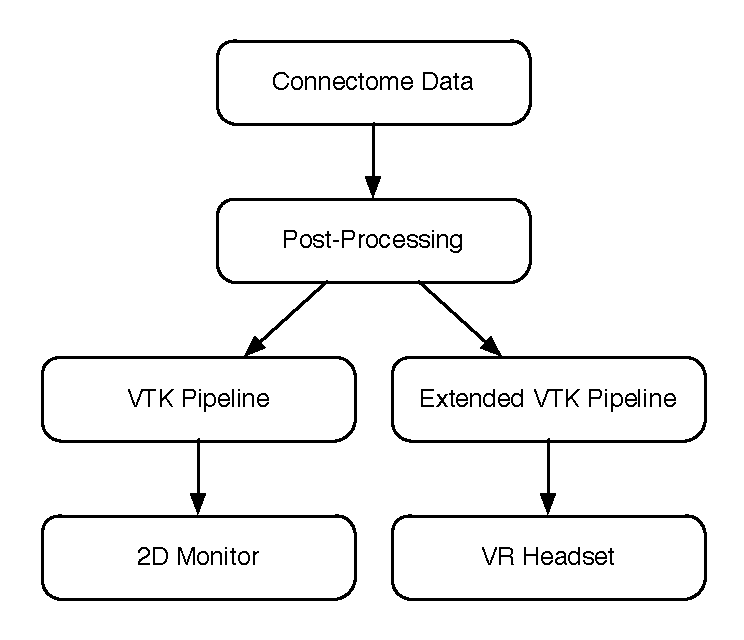
\includegraphics[scale=0.5]{resources/data_pipeline_overview}
    \caption{The Full Pipeline}
    \label{fig:the_full_pipeline}
\end{figure}

With a complete pipeline for VR, Chapter~7 discusses how the system was evaluated. This evaluation identified numerous strengths and weaknesses, and suggestions for further work are explored.

Finally, Chapter~8 concludes by synthesizing findings from each stage in the project, and reviewing the most interesting learning outcomes.

\chapter{Connectome Data}

This chapter discusses why visualising brain data is so important, and why connectome data is suitable source of content for this project. Different experimental techniques for gathering data are compared, with particular attention paid to the type of data that each technique produces. Current data visualisation systems are introduced, with the conclusion that the tractography is particularly well suited to be displayed in 3D. 

\section{Motivation for using Connectome Data}
Mapping and visualising the brain is of considerable academic and practical interest. The brain is thought to be composed of motor, sensory, behavioural state, and cognitive systems \cite{Swanson2003}. Better knowledge about the physiology of the brain can help in understanding these systems. Knowledge of the structure of an individual brain can also be very helpful when diagnosing medical conditions, or planning a surgical procedure \cite{Golby2011}. In either case, the interested parties need to have data, and to be able to draw useful inferences from it. This project aims to work on the second of these challenges: to develop new ways of displaying and interacting with existing connectome data. 

The high quality and availability of connectome data makes it an excellent source of content for visualisation. The Human Connectome Project is a world-class source of data, and thanks to the Open Access Data license terms \cite{HCPAccess2014} all of this content can be obtained free of charge. Imperial College has an active research program in the medical imaging field, and the project has benefited greatly form access to friendly local expertise. As an illustration of this good fortune, Imperial College is one of only four UK universities involved in the Developing Human Connectome Project \cite{DHCPPartners2014}, and over half of the experts\footnote{Kevin Kerdauren, Lisa Koch, Dr Sarah Parisot, and especially Dr Bernhard  Kainz} in the Imperial College team have directly assisted this project. 

\section{Sources of Connectome Data}
An understanding of the processes for generating connectome data is useful, as it influences the resolution and format of the data obtained. 

\subsection{Electron microscopy (EM)} 
EM gives nanometer resolution images of neural structure. This is an ex vivo process, samples must be taken from the brain. EM techniques can give a resolution of \SI{5}{\nm} in the x-y plane, with a \SI{30}{\nm} slice thickness and generate an enormous amount of raw data, of the order of \SI{1}{\pebi\byte\per\mm\cubed} \cite{Jeong2010}.\footnote{That data density is greater than two hundred thousand DVDs per cubic milimeter or, in old money, more than eleven \textit{billion} floppy disks per cubic inch} Due to the high resolution and small sample sizes accommodated by EM techniques, the only connectome to have been completely mapped out by this technique is that of the nematode c.elegans \cite{White1986}.

\subsection{Optical microscopy (OM)} 
OM techniques can be used in conjunction with fluorescent markers to selectively tag and examine brain matter. As with EM, this is done ex-vivo. This approach allows for much larger samples to be analysed, at a resolution of approximately \SI{0.35}{\um} in the x-y plane\footnote{Fluorescent markers allow resolution beyond the Abbé limit without needing metamaterial lenses.}, and with a slice thickness of \SI{100}{\um}. This approach has recently been used to map the entire mouse connectome \cite{Oh2014}. 

\subsection{Magnetic Resonance Imaging (MRI)} 
MRI scans may be used in combination with Diffusion Tensor Imaging (DTI-MRI) as an in-vivo technique for determining larger scale structure. Diffusion of water within the brain is influenced by the structure of the brain matter, since water can diffuse more easily along bundles of nerves than perpendicular to them, and so the diffusion patterns allow local structure to be inferred. The resolution of this technique is typically low, approximately \SI{1}{\mm} in the x-y plane \cite{Westin2002}. A related technique is to detect neural activity, determined as a function MRI measurements of blood-oxygen changes in the brain (fMRI) \cite{Huettel2004}. MRI techniques have been used to map hundreds of human connectomes. 


\section{Storing Connectome Data}
There are no standardised formats for storing raw connectome data, as the form of the data depends on the experimental technique used to obtain it (EM, OM, MRI) and the specific equipment used. For this reason, many imaging tools such as NeuroneJ \cite{NeuronJ2014}, Imaris \cite{Imaris2014}, and Amia \cite{Amira2014} have been developed to work with specific input data formats. Although there is some inter-operability, there is no universal standard data format for imaging data. 

Fortunately, the HCP project does have a set of conventions as to the format and structure of their data. The HCP includes DT-MRI and fMRI measurements from multiple institutions and multiple different scanners, and has been careful to ensure that different data samples may be compared in a valid way \cite{HCP_Logistics_2014}.  In addition to a standard format and organizational structure, the HCP runs de-noising and normalising algorithms on the data. The topic of HCP data is covered in more depth in Section~\ref{sec:the_structure_of_hcp_data}.

Given the large size of connectome datasets, it is sometimes necessary to implement a custom data structure to support certain visualisations. In particular, fast access to the data is essential when working interactively with high resolution images. Previous publications \cite{Jeong2010} have discussed working with a 75GB connectome dataset, stored as an octree in order to enable fast access to the desired parts of the dataset. They also store sub-sampled data at various resolutions in order to allow responsive zooming into the data set and cache data at GPU, CPU and process levels. 

Fortunately, the pre-processing techniques described in Chapter 3 could be used to produce structures with simple geometric structures, and consequently small file sizes. With file sizes less than \SI{10}{\mega\byte}, it is perfectly possible to store the structure in RAM or even in video memory. In the future it may be necessary to investigate more exotic dataset options in order to support more complex content and higher-resolution VR displays.


\section{Visualising Connecome Data}
A number of common visualisations exist for connectome data. Visualisations can be divided into three types: structural, functional and multimodal. Some visualisations, connectivity matrices for example, are equally well suited to display structural or functional information. Other visualisations, such as tractographies, are best suited to displaying structural information. Multimodal visualisations show elements of both structural and functional data. Virtual reality is well suited to display structural information, and so the following visualisations discussed are primarily those for structural or multimodal data.

\subsection{Connectivity Matrix}
A connectivity matrix shows the physical or functional connectivity between different regions of the connectome \cite{Wang2011}. It allows a lot of information to be presented in a single 2D image. However, it does not represent the spatial relationship of the data, and the format in which the axes are ordered may introduce false patterns. 

\begin{figure}[htbp!]
    \centering
    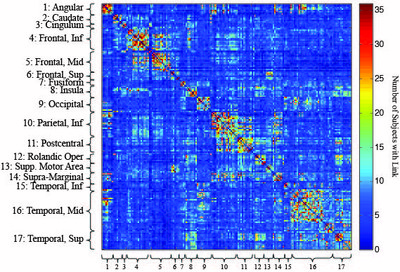
\includegraphics[width=0.5\textwidth]{resources/connectivity_matrix}
    \caption{An alphabetically ordered connectivity matrix. \cite{Wang2011}}
    \label{fig:connectivity_matrix}
\end{figure}

\subsection{Tractography}
Tractography is the process of visualising nerve tracts, bundles of nerve cells. It can provide a very intuitive way of looking at nerve data. It can can require considerable manual editing of opacity, colour and shading in order to bring out the desired features in a tractography image. Without such editing, tractography images suffer from a surfeit of information and can obscure features of interest.

\begin{figure}[htbp!]
    \centering
    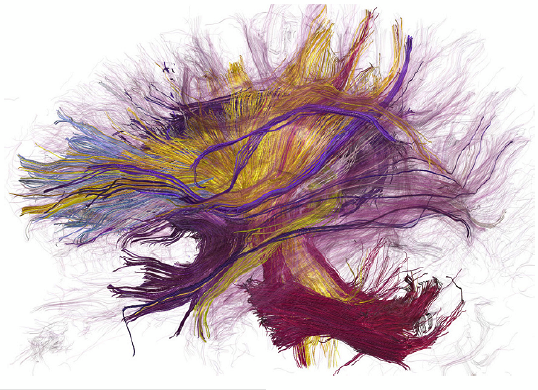
\includegraphics[width=0.8\textwidth]{resources/tractography}
    \caption{Fiber Tractography. \cite{Odonnell2006}}
    \label{fig:tractography}
\end{figure}

Various techniques have been developed for fiber tractography, including the use of tuboids, streamlines and streamtubes to represent the tracts. These techniques can offer a host of advantages including faster rendering times, aesthetically pleasing labelling of tracts, simplified tract junction rendering and good occlusion handling \cite{Petrovic2007}.

\begin{figure}[htbp!]
    \centering
    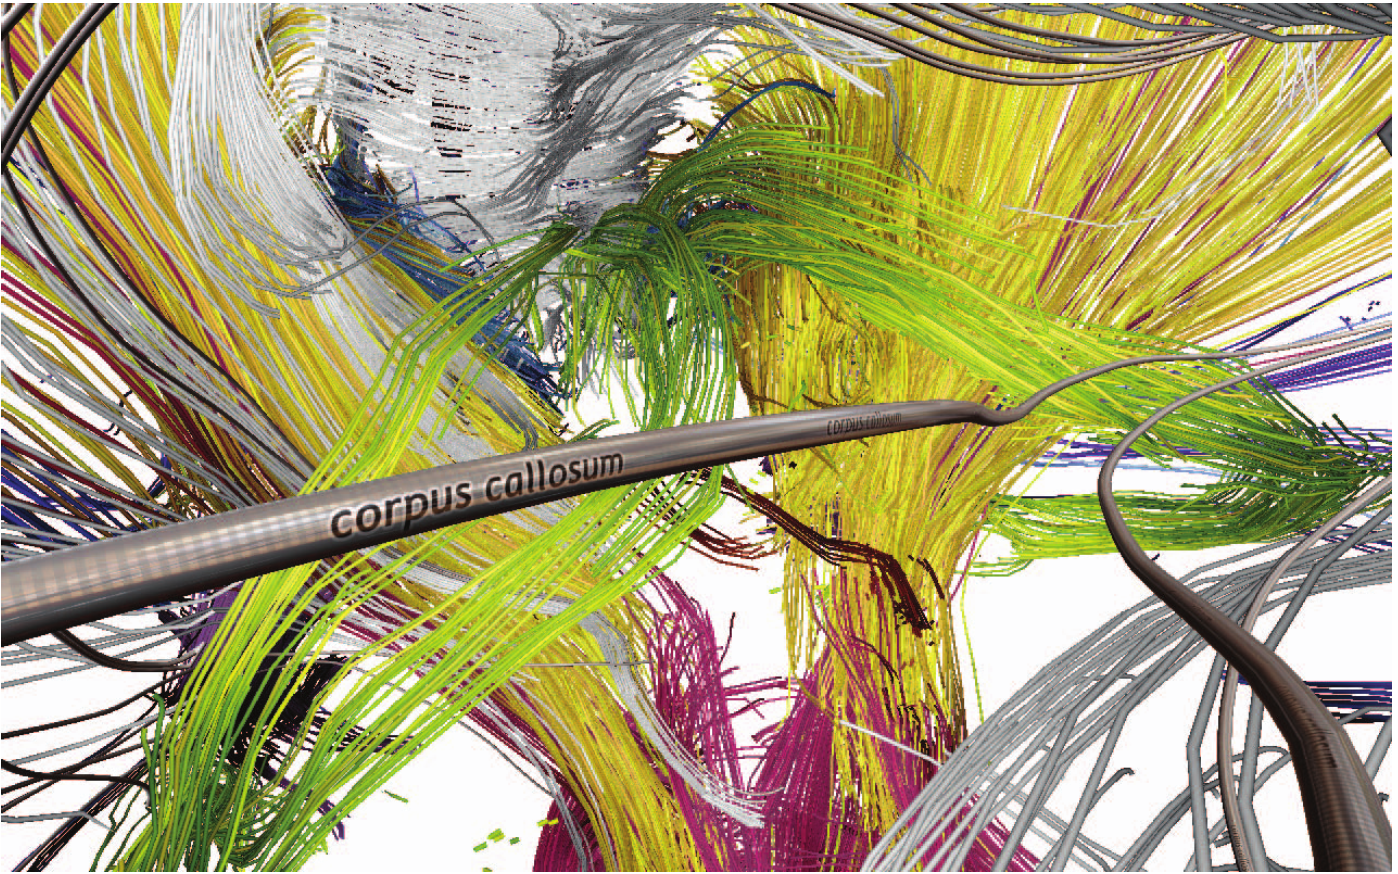
\includegraphics[width=0.8\textwidth]{resources/tuboids}
    \caption{A tractography image using tuboids. \cite{Petrovic2007}}
    \label{fig:tuboids}
\end{figure}

\subsection{Glyph Images}
Glyphs can be used to represent local diffusion tensors in DT-MRI data. The goal of glyph images is to show local diffusion properties as well as larger macroscopic structure. Various systems have been proposed to do this: using ellipsoids \cite{Pierpaoli1996}, colour coded arrows \cite{Peled1998}, opacity mapping \cite{Westin1997}, and hybrid geometric shapes \cite{Westin2002}. 

A spherical glyph represents isotropic diffusion properties, whereas various ellipsoids can represent a local bias towards linear or planar diffusion. Local diffusion can be represented as an ellipsoid or, due to the ambiguity in representing a 3D ellipsoid in a 2D image, as a hybrid shape.

\begin{figure}[htbp!]
    \centering
    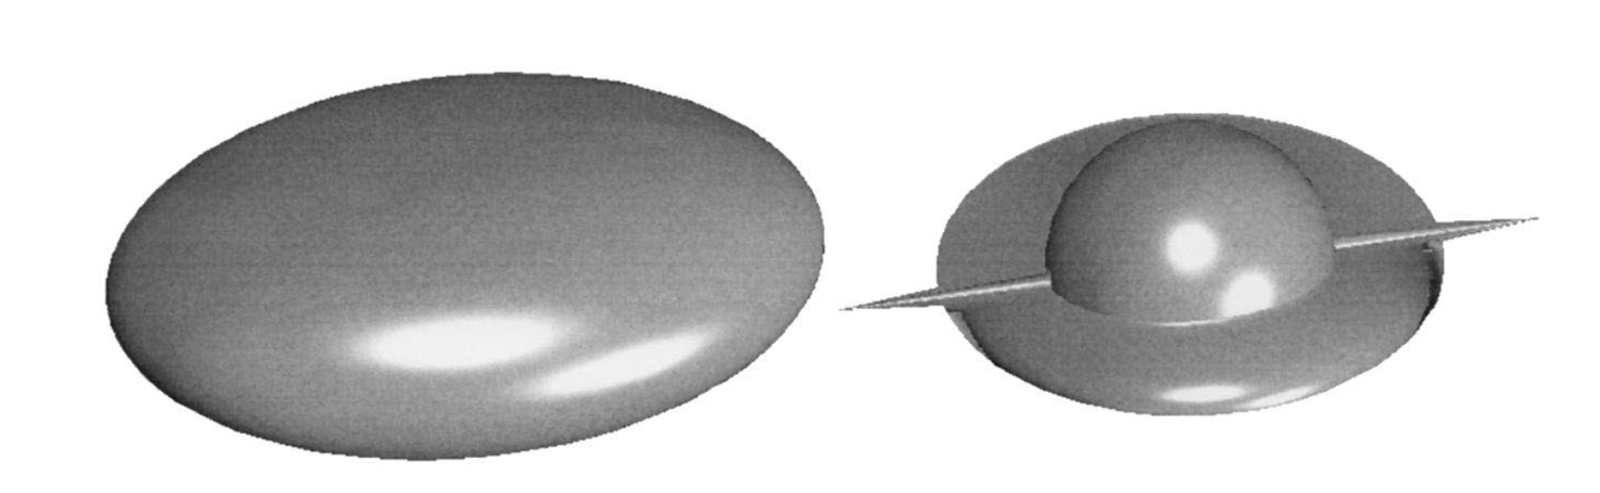
\includegraphics[width=0.6\textwidth]{resources/hybrid_glyphs}
    \caption{Hybrid glyphs representing local diffusivity in DT-MRI data. \cite{Westin2002}}
    \label{fig:hybrid_glyphs}
\end{figure}

The ordered placement of glyphs can introduce patterns not present in the data, prompting research into the positioning of the glyphs, and the use of particle systems to re-position glyphs as a function of interparticle forces \cite{Kindlmann2006}. The benefit of this approach is that the sampling artefacts may be greatly reduced or completely removed from the final image. As can be seen from the figure below, this approach is not without drawbacks, new image artefacts, such at the hexagonal close packing structure, may be introduced by the particle field. 

\begin{figure}[htbp!]
    \centering
    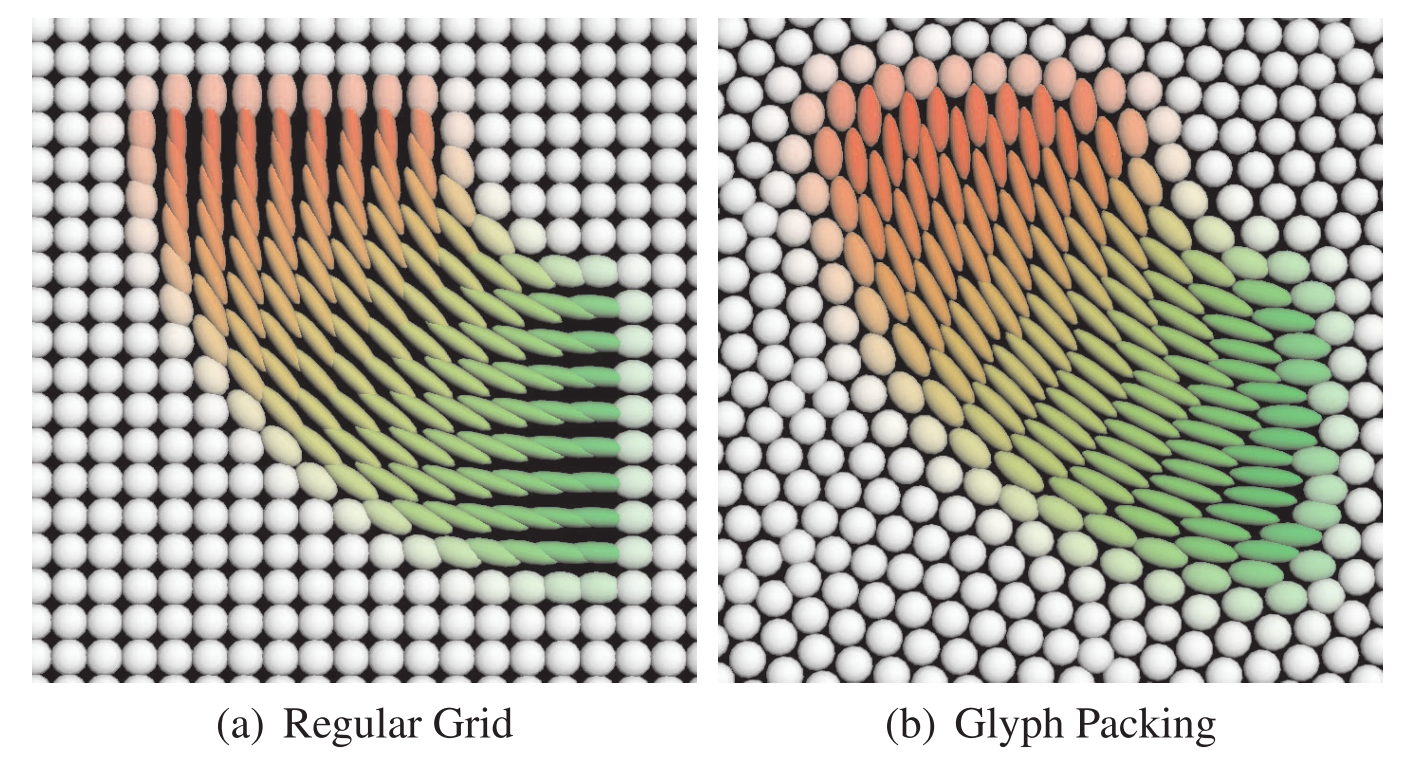
\includegraphics[width=0.6\textwidth]{resources/glyph_packing}
    \caption{Glyph packing. \cite{Kindlmann2006}}
    \label{fig:glyph_packing}
\end{figure}

\subsection{Other Techniques}
In addition to connection matrices, tractographies and glyph images there are a large number of other ways to display connectome data. Graph-based representations can present functional connectivity \cite{Hagmann2008}, but may do so at the cost of reduced anatomical accuracy \cite{Margulies2013}. 

\begin{figure}[htbp!]
    \centering
    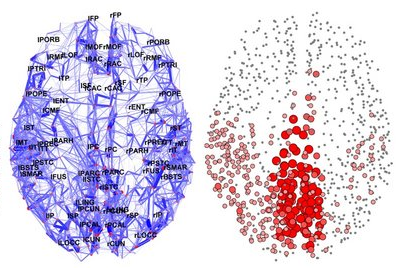
\includegraphics[width=0.8\textwidth]{resources/connectome_graphs}
    \caption{Network structure and interconnection density maps. \cite{Hagmann2005}}
    \label{fig:connectome_graphs}
\end{figure}

The Glass Brain project has developed a multimodal technique for combining structural and functional data \cite{GlassBrain2014}. This type of representation may be useful as it gives anatomical context alongside functional information. 

\begin{figure}[htbp!]
    \centering
    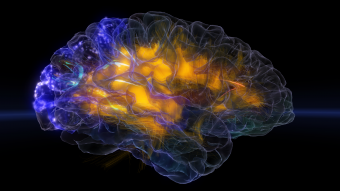
\includegraphics[width=0.8\textwidth]{resources/glass_brain}
    \caption{A Glass Brain visualisation. \cite{GlassBrain2014}}
    \label{fig:glass_brain}
\end{figure}

\section{Summary}
Human DTI-MRI data from the Human Connectome Project was chosen for use in this project due to it's availability, quality, and the importance of the subject matter \footnote{With apologies to the nematode c.elegans, and the various mouse-brain connectomes that were candidates for this role.}. 

The choice of visualisation system was a more complex issue. For the purpose of this project, it is useful to note that, with the exception of the connection matrix, all of the visualisation techniques for connectome data attempt to represent 3D (or greater dimensionality) information in a 2D image. This is has two important consequences:
\begin{enumerate}
\item It shows that there is a need to display 3D data.
\item It shows that, in many cases, three dimensional processing and rendering is already being done.
\end{enumerate}

2D representations have a number of advantages. The sampling methods used in measuring the connectome data gather 2D data, the full connectome structure being reconstructed from many planar slices. Relatively little processing is needed in order to convert an array of data into a viewable image, and so a 2D visualisation can be a very fast way to look at raw data. The ‘flat’ nature of 2D images makes them very simple to display or print, to transport and to store. 

Pseudo-3D images are frequently used. These use either colours or symbols to represent out-of-plane structure. Alternatively, they may show a 3D representation of the connectome, rendered into a 2D picture. Using this definition of ‘pseudo-3D’, all of the above visualisation techniques (except the connection matrix) would fall into this category. 

Full 3D images seem very well suited to visualising connectome data. Given that there is a need to display 3D data, and that much of the data is already processed and rendered as a 3D model, it seems natural to displaying it natively in 3D. If the only objections to 3D visualisations is the expense of current 3D hardware \cite{Margulies2013} then a proliferation of cheap consumer hardware may remove this barrier in the near future.

Given these considerations, all of the 3D visualisation styles were candidates for the project. The tractography was selected due to it's intuitive and elegant nature. Of all of the styles discussed, it is the one most easily understood by non-experts, and so suitable content for a wide target audience.

\chapter{Post-Processing}

This chapter discusses the the data-wrangling necessary to convert HCP data into a suitable input format for the VTK pipeline. The HCP dataset is examined using ITK-SNAP, and the DTI-MRI data selected as a starting point. The format of the HCP data is explained, and an intermediate data format (legacy vtk) is chosen. The HCP data is then processed using Camino, ITK-SNAP, MITK, and MATLAB in order to obtain a tractography, and a cortical surface and dense surface mesh. A Blender plugin is developed in order to import and examine the VTK mesh, and the relative benefits of each post-processed content are discussed.  


\section{The Structure of HCP Data} \label{sec:the_structure_of_hcp_data}
HCP data is intended to be a standard format, allowing for comparison between hundreds, eventually thousands, of individual human connectomes. Chapter 2 discussed the different types of connectome data, and concluded that the project should use MRI-DTI data. Figure~\ref{fig:hcp_full_data_set} shows that much of the HCP dataset contains a wide variety of different experimental data, and that the decision to focus on MRI data narrows the search space down considerably.

\begin{figure}[htbp!]
    \centering
    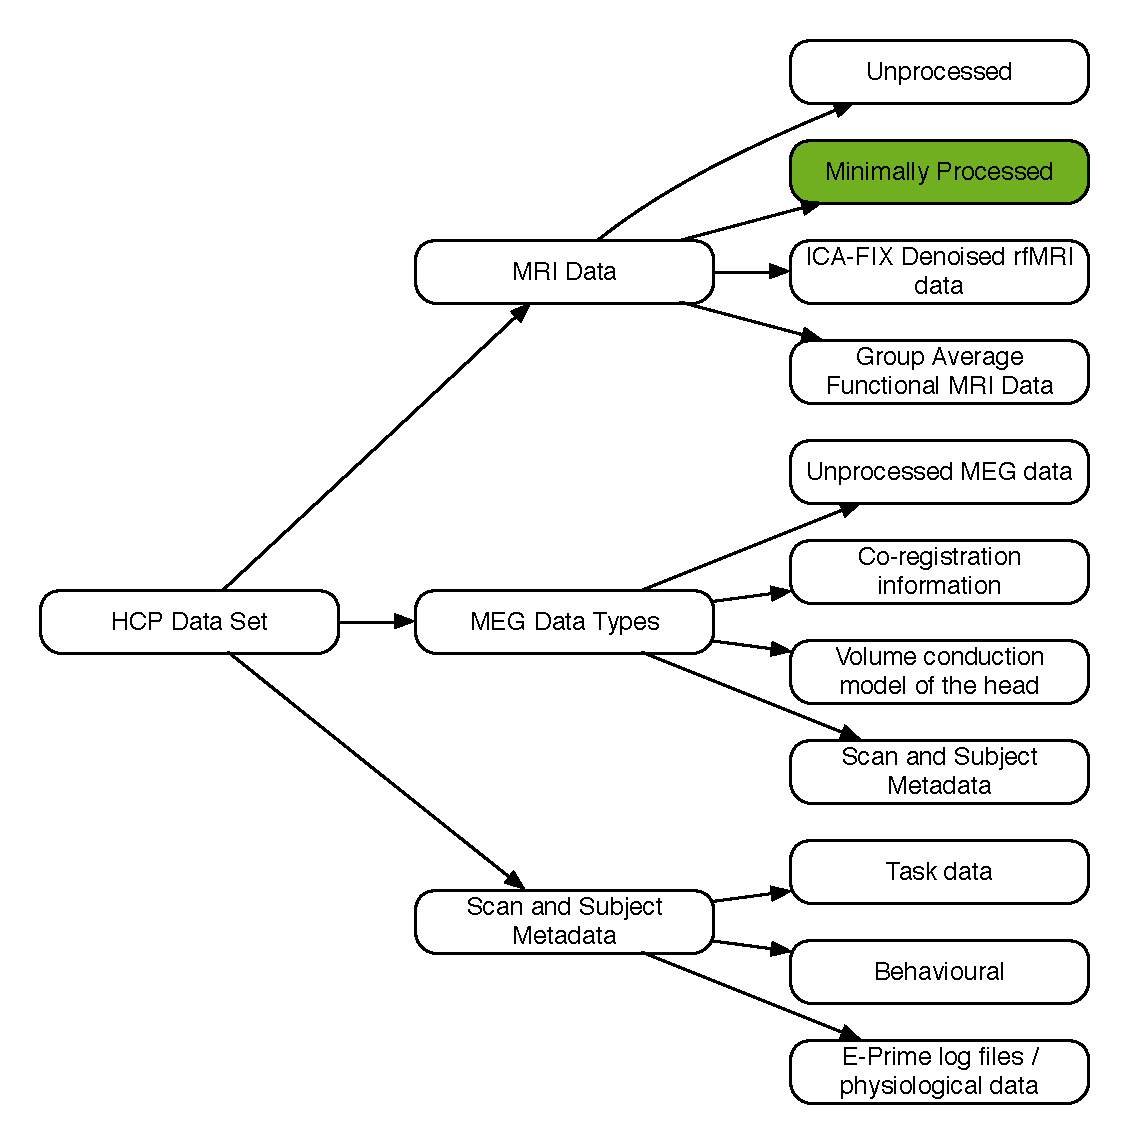
\includegraphics[width=0.8\textwidth]{resources/hcp_full_data_set}
    \caption{Components of a sample HCP Data Set.}
    \label{fig:hcp_full_data_set}
\end{figure}

The project needs access to structural information in a format that can be imported in VTK. The MRI data in the HCP dataset cannot be directly imported as desired. The following section describes how the HCP data is stored, and consequently how it can be processed into a useful intermediate format. This is done in two ways: a tractography is generated from the structural MRI-DTI CIFTT data, and a cortical surface is obtained by converting a GIFTI surface file. 

\subsection{NIfTI Data}
The main format of the HCP data is Neuroimaging Informatics Technology Initiative (NIfTI) format. Recent data is in the NIfTI-2 format, an extension that uses \SI{64}{bit} storage and addressing to allow for larger data sets with more precision. To the explorer browsing an HCP data set, these are the $\ast.nii$ files \footnote{or sometimes compressed (gnu-zipped) $\ast.nii.gz$ or tar-archived $\ast.nii.tar$ files.}. The NIfTI format holds data as a 4D matrix (x, y, z and time), as well as containing meta-data in a header. Conceptually, data can be extracted from NIfTI format by taking a 3D matrix 'slice' out of the set, to get voxel data for a specific point in time. 

\subsection{CIFTI Data}
CIFTI is a related data format to NIfTI, more of a \textit{flavour} of NIfTI than a separate file format and so has the same file extensions. CIFTI files reference other files, frequently GIFTI surfaces, to specify relative vertex and voxel positions. CIFTI files can contain dense or sparse matrices, and are often used to store many different volumes that each correspond to a different anatomical region \cite{WorkbenchGlossary2014}. 

\subsection{GIFTI Data}
Following widespread adoption and success of the NIfTI format, the Geometry Informatics Technology Initiative were set up to create a new standard format to store geometrical surfaces. The result was the GIFTI format, designed to store a variety of data types including surfaces, measurements and labels \cite{Harwell2011}. These are the $\ast.gii$ files in the HCP dataset, and they mostly represent surfaces. Figure~\ref{fig:connectome_gifti} shows the native, midthickness, inflated and very inflated cortical GIFTI surface files from HCP data, viewed in The Connectome Workbench.

\begin{figure}[htbp!]
    \centering
    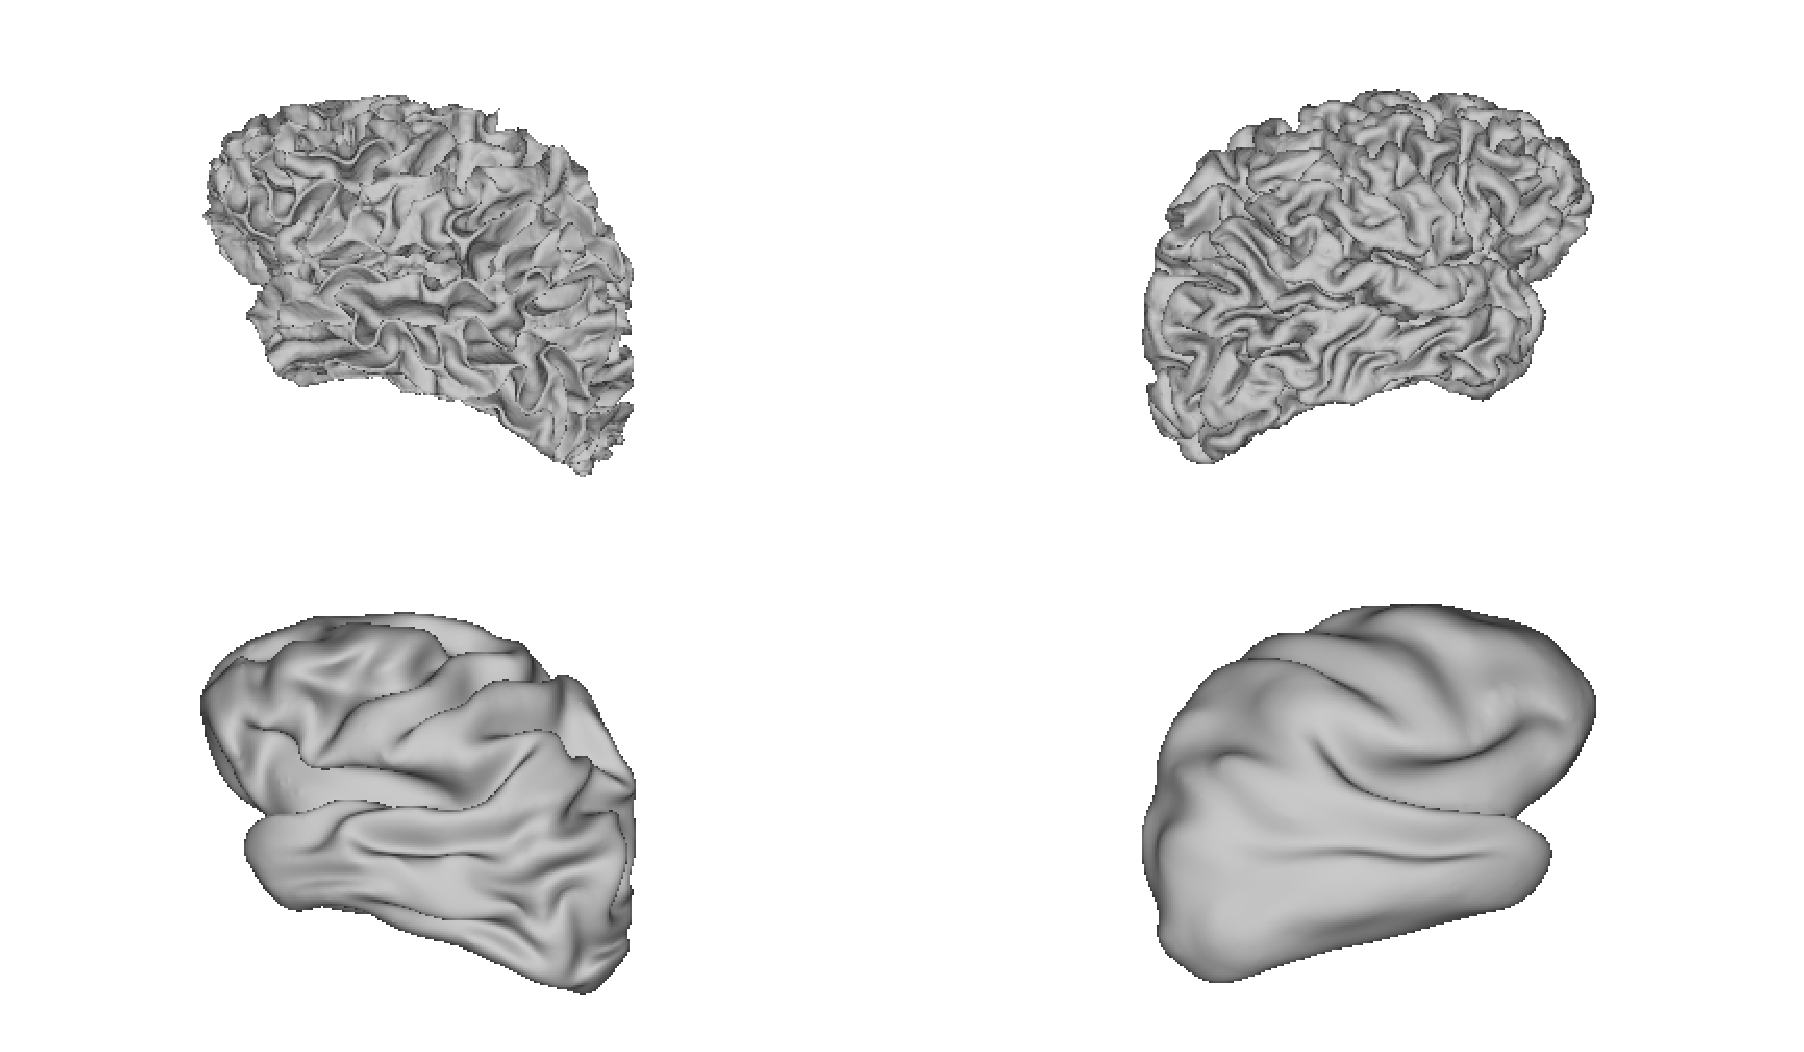
\includegraphics[width=0.8\textwidth]{resources/connectome_gifti}
    \caption{Components of a sample HCP Data Set.}
    \label{fig:connectome_gifti}
\end{figure}

\section{Choosing an Intermediate Format}
\label{sec:choosing_an_intermediate_format}
Before an intermediate format had been chosen, a number of 3rd party programs were investigated for reading and converting HCP data. MeshLab \cite{MeshLab2014} was found to be an excellent mesh conversion tool, but could not load any of the GIFTI or NIFTI data sets. Medinria \cite{MedInria2014} could work with the available data sets but was better suited to viewing content than converting it. With assistance from Dr Kainz, MITK \cite{MITK2014} was used to select a region in a CIFTI file using an image intensity threshold, and then outputting the selection as a vtk mesh. This was a significant step forward: the vtk data format was perfectly compatible with the Visualisation Tool Kit, and the resulting mesh was the first 'real' connectome data visualised on the Rift.

The vtk data format proved to be very suitable for this project for a number of reasons. On a practical basis, it was known to work with VTK, and so could provide the Rift with suitable content for demonstrations. Further research showed that it was a well established format \cite{VTK_file_formats}, and the it's wide support made it a suitable intermediate format. In addition to these points, the 'legacy' VTK format holds data in a simple, plain text structure. This was a very strong reason for using the format, as it allowed human inspection of the mesh data. 

\begin{lstlisting}[label=vtk_data_structure, caption=The structure of data in a legacy .vtk file.]
# vtk DataFile Version 2.0  // # vtk DataFile Version 3.0
Really cool data            // vtk output
ASCII | BINARY              // ASCII
DATASET type                // DATASET POLYDATA
...
POINT_DATA n                // POINTS <number> float
...
CELL_DATA n
\end{lstlisting}

Listing shows the header specification from \cite{VTK_file_formats} with comments illustrating vtk parameter values in a real dataset. Information such as the number of points in the mesh proved to be very useful when debugging the VTK render output.

\section{Data conversion using MITK}
As mentioned in Section \ref{sec:choosing_an_intermediate_format}, MITK was used to export a region of a CIFTI cortical data file as a 3D mesh. This process is shown in Figure \ref{fig:MITK_conversion}. The process involved selecting a volume in the original data file using a thresholding function, and then creating a mesh from the selected region. Once that was done, the mesh could be exported as a vtk file.

\begin{figure}[htbp!]
    \centering
    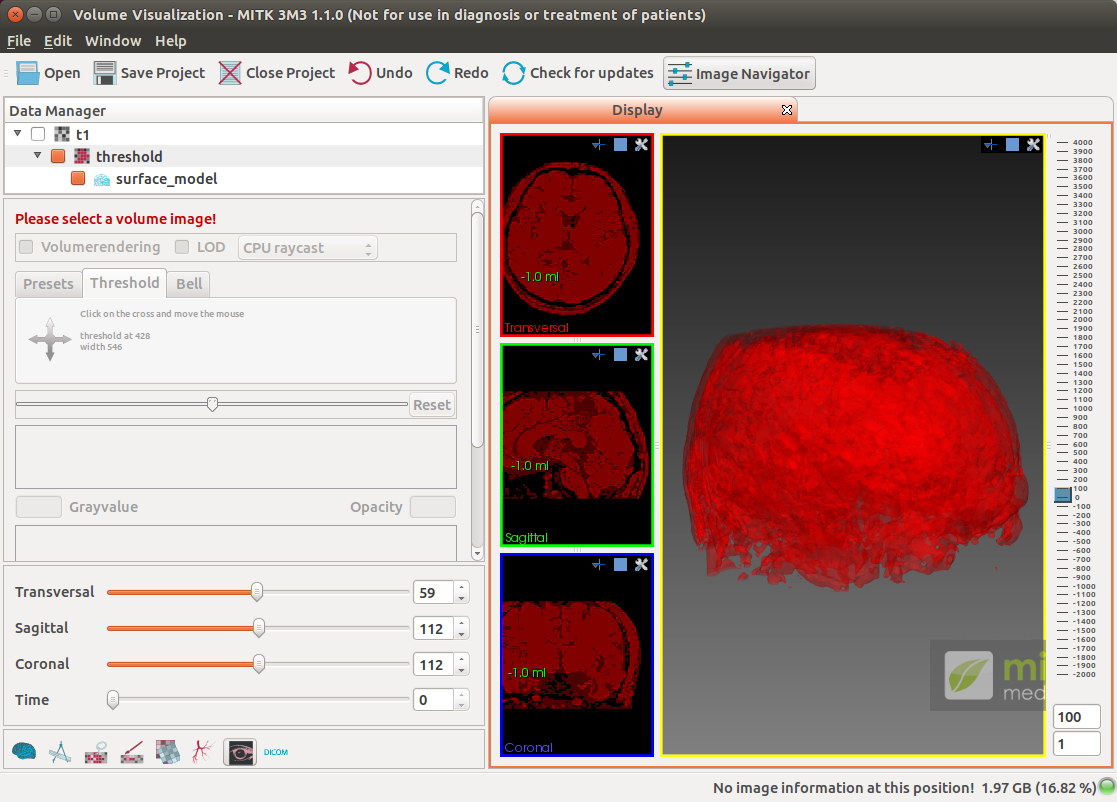
\includegraphics[width=0.8\textwidth]{resources/MITK_conversion}
    \caption{Converting CIFTI data to vtk using MITK.}
    \label{fig:MITK_conversion}
\end{figure}

This approach had two significant problems. Firstly, with little experience in working with this type of content it was difficult to choose a meaningful threshold and the resulting mesh was correspondingly arbitrary. Worse still, this approach produced a noisy, complex mesh that took approximately \SI{100}{MB} of ASCII vertex positions to fully express. Due to the noise in the image, the size of the mesh did not add any information, but it did cause significant problems with the render-speed. These problems are discussed in the Results Chapter.

\section{Data conversion using MATLAB}
After learning more about the HCP data structure, it was understood that certain GIFTI files in the HCP data set already contained cortical surface representations. This would be perfect demonstration content and would have none of the size or noise issues of the MITK-converted data-set. 

\begin{figure}[htbp!]
    \centering
    
\includegraphics[width=0.8\textwidth]{resources/placeholder}
    \caption{Converting GIFTI data to vtk using MATLAB.}
    \label{fig:MATLAB_conversion}
\end{figure}

Converting GIFTI format data to vtk proved to be a challenge. Shortly after the idea had been abandoned, Dr. Sarah Parisot returned from a vacation and insisted to me that such a conversion must be possible. With her support, and her access to MATLAB, we were able to use Professor Chris Rorden's MATcro conversion tools to convert the HCP GIFTI surface files into VTK polydata meshes. These mesh files were only \SI{6}{MB} in size, compared with the \SI{100}{MB} size of MITK-conversions, which translated into quick rendering and a high frame rate when displaying the content on the Rift.

\section{Data conversion using CAMINO}
The initial aim of the project had been to display complex


\section{Bonus: Developing a Blender Plug-in}

\chapter{The Visualisation Tool Kit}
This chapter introduces the Visualisation Tool Kit (VTK), explaining why VTK is an appropriate tool for the project. A simple VTK rendering pipeline is then described, to provide context for subsequent developments. The simple pipeline is modified to work with real connectome data, and additional manipulation tools are added. Finally, the pipeline is modified so that it can produce stereoscopic image pairs.

\section{Introducing VTK}
VTK is a software system for 3D computer graphics, image processing, and visualisation. For the purpose of this project, it's defining characteristics are:
\begin{enumerate}
\item \textbf{It is an open source project, freely available via GitHub.} This proved to be very useful, as the software could be cloned and built immediately and without needing to pay any license fees. The C++ source code was a useful supplement to documentation and tutorials, since it allowed the source to be searched or 'grep-ed' and read. Access to the source code proved to essential when the project needed to extend VTK functionality via subclassing. 
\item \textbf{It is mainly written in C++.} This was useful at a practical level, as the MSc course had provided an introduction to C++. The development model of VTK is to provide core functionality in C++ and then support other languages such as Java and Python using wrappers. This model meant that any functionality added to VTK during this project could be extended to other languages through automatically generated wrapper code.
\item \textbf{It is under active development, and used extensively by the medical imaging community.} The active development of VTK was useful as it meant that there was a substantial volume of documentation and forum material surrounding the software. This meant that it was often possible to learn from past examples and avoid well known problems. The development of VTK by the medical imaging community also meant that VTK could work with medical data formats (well... sort of. Only in 6.x, which I couldn't use) and that there was a known user group who would be interested in any useful developments.
\item 
\end{enumerate}

Developed by Kitware Inc., VTK works well with CMake, and can run on all of the major OS platforms. VTK is also used to do all of the Visualisation work inside Paraview, as well as other notable open-source projects including 3DSlicer.

\section{The VTK Pipeline}
The VTK pipeline is illustrated in Figure~\ref{fig:vtk_pipeline}, with a VTK cone primitive in place of more complex data. In order to use connectome data, it is necessary to load the data as a source. The source must be in a format the VTK can then map to primitives, which places a restriction on the nature of the input data.

Some important components are hidden in this basic pipeline: neither the light nor the camera in the render scene are	 shown. These are both contained in the Renderer, and if not explicitly set then VTK initializes them to default values. This behaviour is simultaneously a great strength and a great liability: it allows a rendering pipeline to be set up very quickly, but it does require that the user be familiar with the pipeline and the various default settings.

\begin{figure}[htbp!]
    \centering
    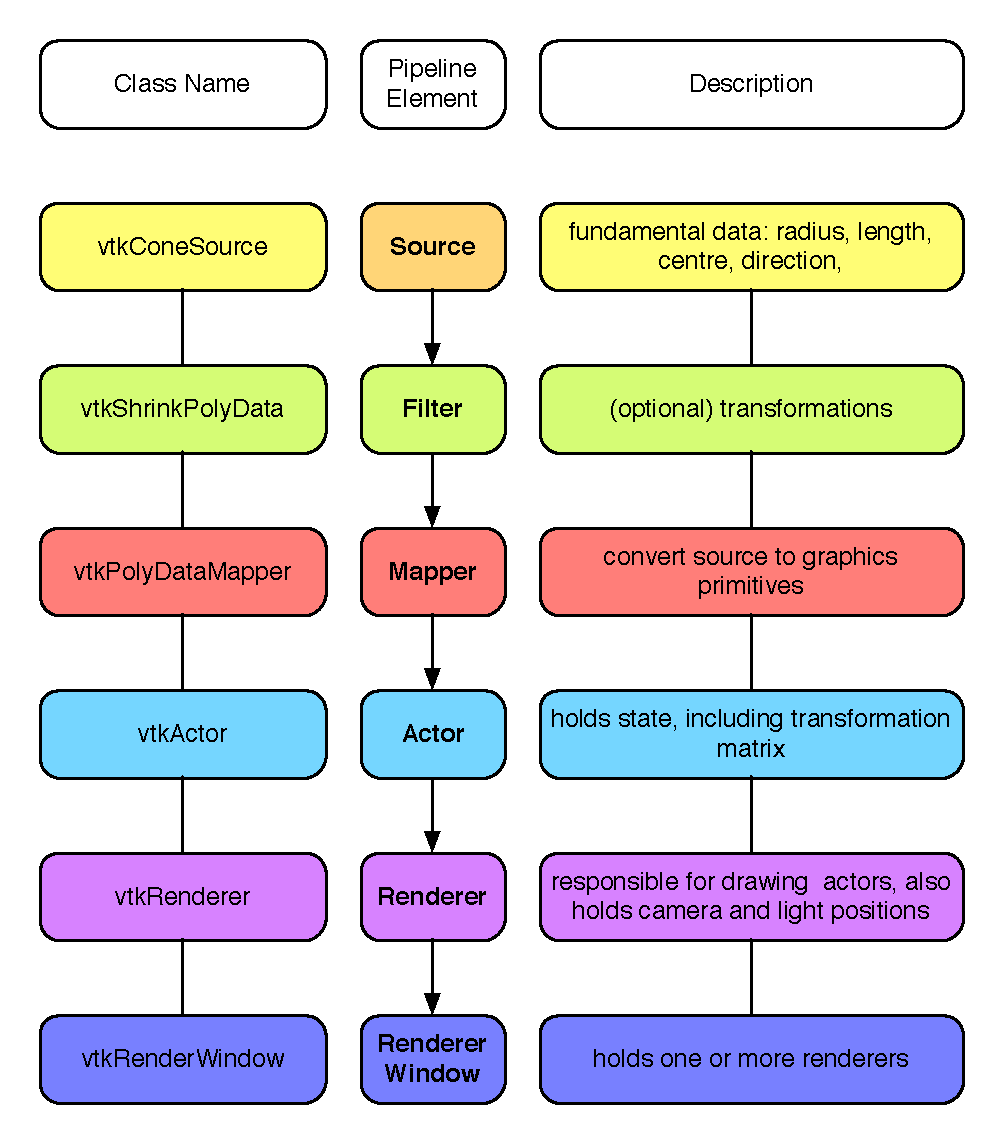
\includegraphics[width=1\textwidth]{resources/vtk_pipeline}
    \caption{The Basic VTK Pipeline for a Cone Primitive}
    \label{fig:vtk_pipeline}
\end{figure}


\section{Complex Data Sources}
Loading and rendering connectome data can be relatively straightforward. Compatibility with a wide range of input data formats was one of the reasons why VTK was chosen as the tool kit to use for the project.

\begin{figure}[htbp!]
\centering
\begin{subfigure}{0.5\textwidth}
    \centering
    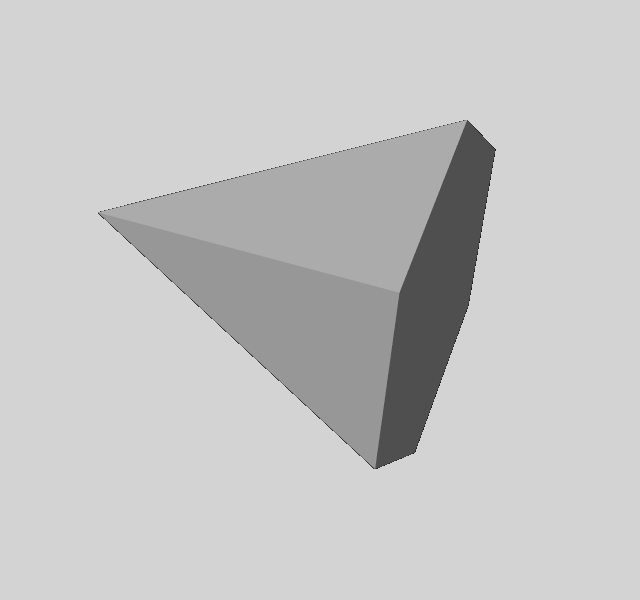
\includegraphics[width=0.8\linewidth]{resources/cone}
    \caption{Cone}
	\label{fig:sub1}
\end{subfigure}%
\centering
\begin{subfigure}{0.5\textwidth}
    \centering
    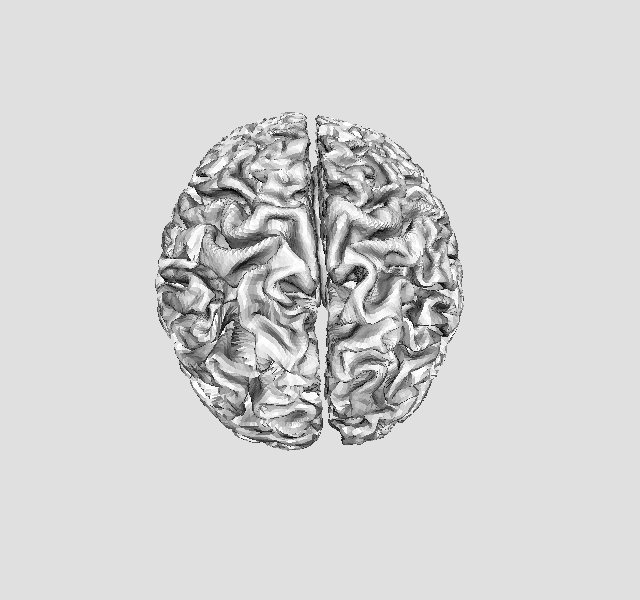
\includegraphics[width=0.8\linewidth]{resources/cortical_surface}
    \caption{Cortical Surface}
	\label{fig:sub2}
\end{subfigure}    
    \caption{HCP Data Rendered Using VTK}
    \label{fig:data_sources}
\end{figure}


VTK can read in a large number of file formats including NIfTI (.nii) and VTK's own '.vtk' extension. During testing, a cortical surface data set was used, stored as a \SI{107}{\mebi\byte} '.vtk' file. This was easily read with a vtkReader object and mapped in as polydata. The impact of the large file size, or more accurately the complexity of the object to render, on rendering speed should not have been sufficient to cause visible latency.

\section{Interaction and Callbacks}
Rendering a scene in a continuous loop is a very computationally inefficient technique. It is much better to only re-render the scene in response to a trigger such as a keypress or mouse movement event. Mouse movement is such a common interaction style that it is implemented in VTK using the vtkInteractor object, and even comes with a number of default styles including 'trackball' and 'joystick' modes. Responding to key presses was implemented using a listener  / callback paradigm. VTK conveniently deals with all aspects of logging and queuing the key press, and can trigger a function in response to the event. 

A virtual reality system is a little more demanding than a normal 2D interface since the viewpoint may be continuously moving as the user's head changes position. Ideally the scene would be re-rendered in response to very small changes in head position. The sensors in the HMD report the head position in floating point units, and the precision is so high that any two position queries show some difference. It would be trivial to set thresholds for the pitch, roll, and yaw that would trigger a re-render of the viewpoint but this solution contains it's own problems. Most significantly, if a \SI{5}{\degree} change in head pitch is required to trigger a re-render of the scene, then the scene is always going to jump a minimum of \SI{5}{\degree} in response to changing head position. An attractive alternative solution is to use a clock timer in order to re-render at a fixed frame rate, irrespective of the user's head position. If the system can cope with rendering imagery at \SI{60}{\Hz} then a \SI{16}{\ms} timer should result in smooth scene movements independent of the user's movements.

Interaction for a naive stereo system holds one additional terror. VTK's automatic mouse interactors operate per-renderer, but a the stereo cameras need to be updated simultaneously to prevent the user going cross-eyed. Fortunately, VTK provide a snippet of Python code illustrating how to work around this restriction. The trick is to ensure that the active mouse interaction affects all cameras in the scene, using temporary variables to store each interactor id. 

\section{Rendering Stereo Images}
Rendering stereo images is beautifully intuitive. Stereoscopic 3D involves viewing different images with each eye in order to get an impression of depth. Using VTK, it is possible to create two cameras and position them as if they were eyes viewing objects in the scene. For comfort, the images should be generated using a camera spacing similar to that of the user's Inter-Pupillary Distance (IPD)\footnote{for most of the population this can be safely approximated as \SI{62}{\mm}} although nearby objects in a scene can cause discomfort even when the camera separation is set correctly. The reason for this is that the human visual system copes badly with extreme vergence - it is difficult to focus on an object very close between the eyes\footnote{and for exactly the same reason it is uncomfortable when 3D movies insist on bringing things too close to the audience!}. 

VTK does contain a 'stereo camera' class, but the documentation for this is rare, and implementation usually involves colour anaglyph or interlaced stereographic image systems. The rift needs stereo input to be available in a 'side-by-side' format, and the most basic method of implementing this was to use two separate renderers, each of which was associated with an independent monoscopic camera 

\todo{blender scene image of the stereo rendering layout}

\chapter{Displaying Images on the Rift DK1}
This chapter provides a very short introduction to the concept of virtual reality in order to provide context for the Oculus Rift DK1. The hardware of the DK1 is introduced and then the key areas are examined. The first of these is the head-mounted sensors, which enable position tracking and viewpoint interaction. The second key area is the lens system, and the optical deformation that must be corrected for during the render process in order to display content to the user. 

\section{An Introduction to Virtual Reality}
Virtual Reality (VR) refers to the visualisation of an artificial environment. This distinguishes it from Augmented Reality (AR) where the user simultaneously experiences real and virtual environments. The Oculus Rift is a VR device since it completely shuts out any view of the real world, whilst Google Glass is an AR device since it shows information as an overlay of the real world.

VR is an attractive way of getting stereoscopic 3D. The current generation of virtual reality hardware offers high-resolution, immersive, stereoscopic 3D performance at a price of a high-end LCD monitor. 

Various VR and AR systems were investigated, as shown in the Mind Map below. Many of the products investigated have been designed for consumers to watch films or play games. These systems do not include any positional feedback, since they are not designed to give an immersive experience but rather to act as a personal cinema screen. Another sub-set of the systems were designed for industrial or military use. These systems would potentially provide the desired performance, but were either prohibitively expensive or completely unavailable for purchase. 

\begin{figure}[htbp!]
    \centering
    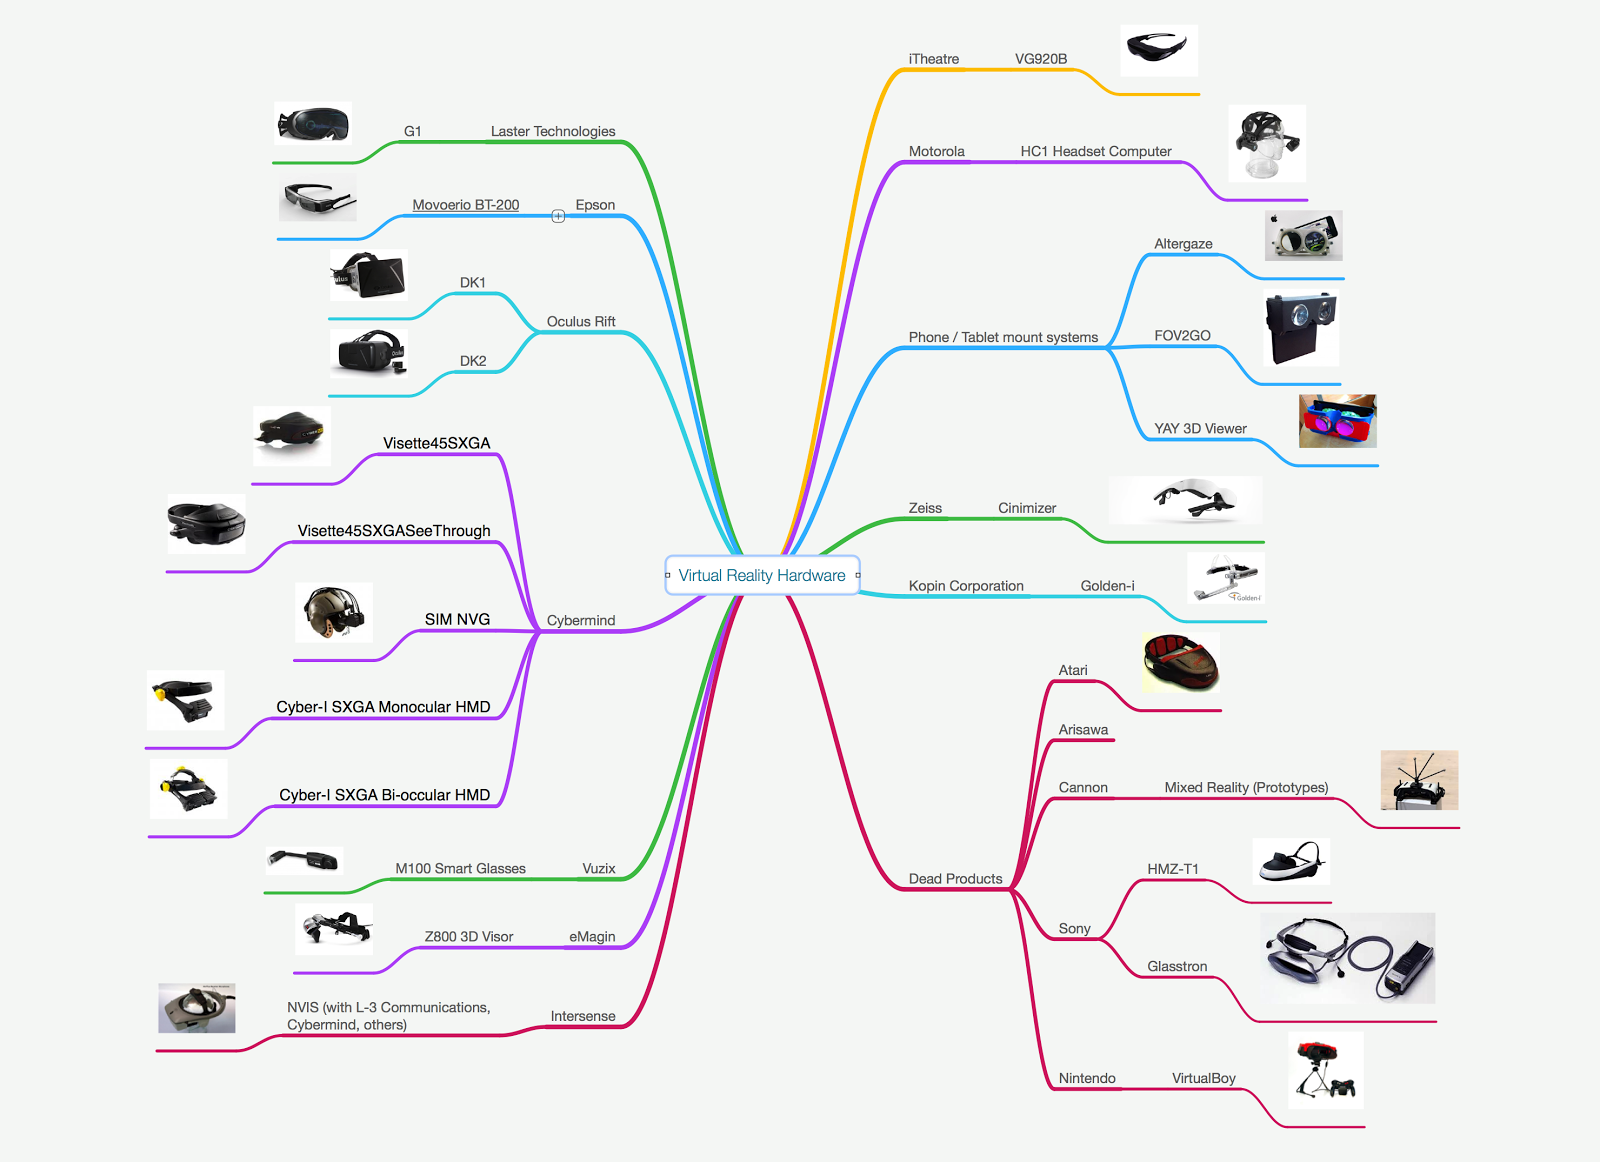
\includegraphics[width=0.8\textwidth]{resources/vr_headsets}
    \caption{AR and VR Products (an incomplete set)}
    \label{fig:vr_headsets}
\end{figure}

The OculusRift DK1 was found to offer the highest performance at the lowest cost. The DK1 is also a suitable system due to the active development of the SDK, and large open source community surrounding the project. Future development of the SDK and the forthcoming release of the compatible DK2 should enable the project to be forward compatible with future hardware, if that is required.
\section{Related Projects}
There is no other known project using an Oculus Rift for the visualisation of connectome data. There have been a small number of projects on using Virtual Reality for connectome visualisation. 

The most similar known projects are:
\begin{itemize}
  \item \textbf{The Dynamic Connectome}, part of the CEEDS project: real time, visualisation of neural activity \cite{ceeds2014}.
  \item \textbf{The Glass Brain Project}: real time, visualisation of neural activity \cite{GlassBrain2014}.
  \item Project work at Aachen University \cite{Rick2011}: using MOCAP and a CAVE virtual environment to interactively view a connectome with dynamic clipping \cite{ceeds2014}.
  \item Project work at Purdue University \cite{Chen2011}: using a CAVE virtual environment to view a connectome.
  \item \textbf{Brainder} \cite{brainder2014}, Dr Anderson Winkler’s excellent blog on FMRI and Blender rendering.
\end{itemize}


The Glass Brain Project uses a Unity 3D model of the brain, though it subsequently renders a 2D image from the model for display on LCD monitors. As such it does not obtain many of the benefits of the 3D model, nor have to face the challenges of displaying images in 3D.

The Dynamic Connectome project and the Aachen University and Purdue University projects use computer assisted virtual environment (CAVE) virtual reality rooms with multiple projectors rather than a head mounted display (HMD) system as proposed here. Such a system removes the requirement to wear bulky headgear, but instead requires a multi-projector system and dedicated room of projection screens. In addition to these requirements, the CAVE systems do not typically show 3D, nor do they update the view based on the user’s precise head position.

The Brainder project uses the open source ‘Blender’ 3D modeling software to ray trace brain models, primarily for use as 2D illustrations. Although the goals of Brainder are different from this project, the existence of (relatively) simple 3D brain models may be a useful asset. 



\section{Introducing the Rift DK1}
\section{Collimating Optics and Software Compensation}
\section{Integrated Sensors and the HMD}

\chapter{Extending VTK}
At the end of Chapter 4, the VTK pipeline had been configured so that connectome data could be loaded, manipulated using interactors, and rendered as a stereo-pair. Chapter 5 then noted that the collimating lenses in the Rift would distort any images sent to the rift. This chapter describes how image processing in software can be used to compensate for optical artefacts, and how GLSL shaders can be used with VTK in order to apply the image correction in real time. 

\section{The Need for Shaders}
\label{sec:need_for_shaders}
Before diving into the details of implementation, it is useful to understand the motivation for using image processing, and shaders in particular. 

\subsection{Using optics to correct for distortions}
The undesirable deformations introduced by the Rift lenses could be corrected by using additional optics. Two corrections would be required: firstly to compensate for the pincushion deformation whilst maintaining the extended field of view, and secondly to reduce the chromatic aberrations caused by dispersion of light in the lens glass. The pincushion distortion could be eliminated by using a lens doublet, and a central aperture \cite{Brainerd2004}. The problem of chromatic aberration could be dealt with by means of achromatic lenses or by using extra-low (EL) dispersion glass in the lens system \cite{Davis2014}. 

These solutions would be appropriate for high-end camera lenses, as shown in Figure \ref{fig:camera_lens}, but are completely impractical for the Rift headset. The lenses in the Rift, shown in Figure \ref{fig:rift_lens}, are designed to be small, cheap and robust. Any optical correction system would involve multiple lenses (increased weight), spacing (increased size), require rigid positioning (increased fragility) and require expensive EL glass (cost).

\begin{figure}[htbp!]
\centering
\begin{subfigure}{0.5\textwidth}
    \centering
    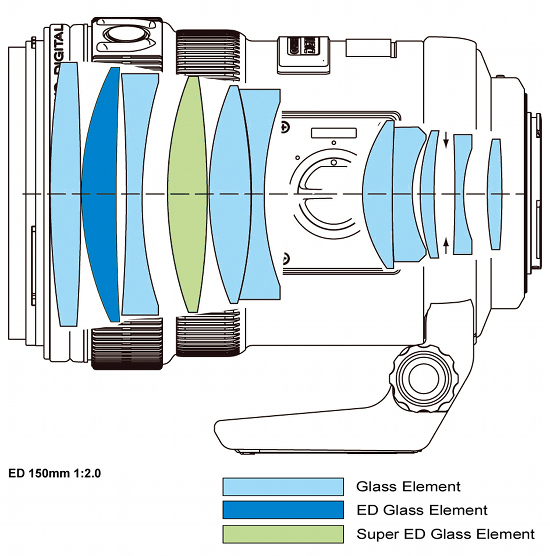
\includegraphics[width=0.5\linewidth]{resources/camera_lens}
    \caption{Camera lens (lenstip.com)}
	\label{fig:camera_lens}
\end{subfigure}%
\centering
\begin{subfigure}{0.5\textwidth}
    \centering
    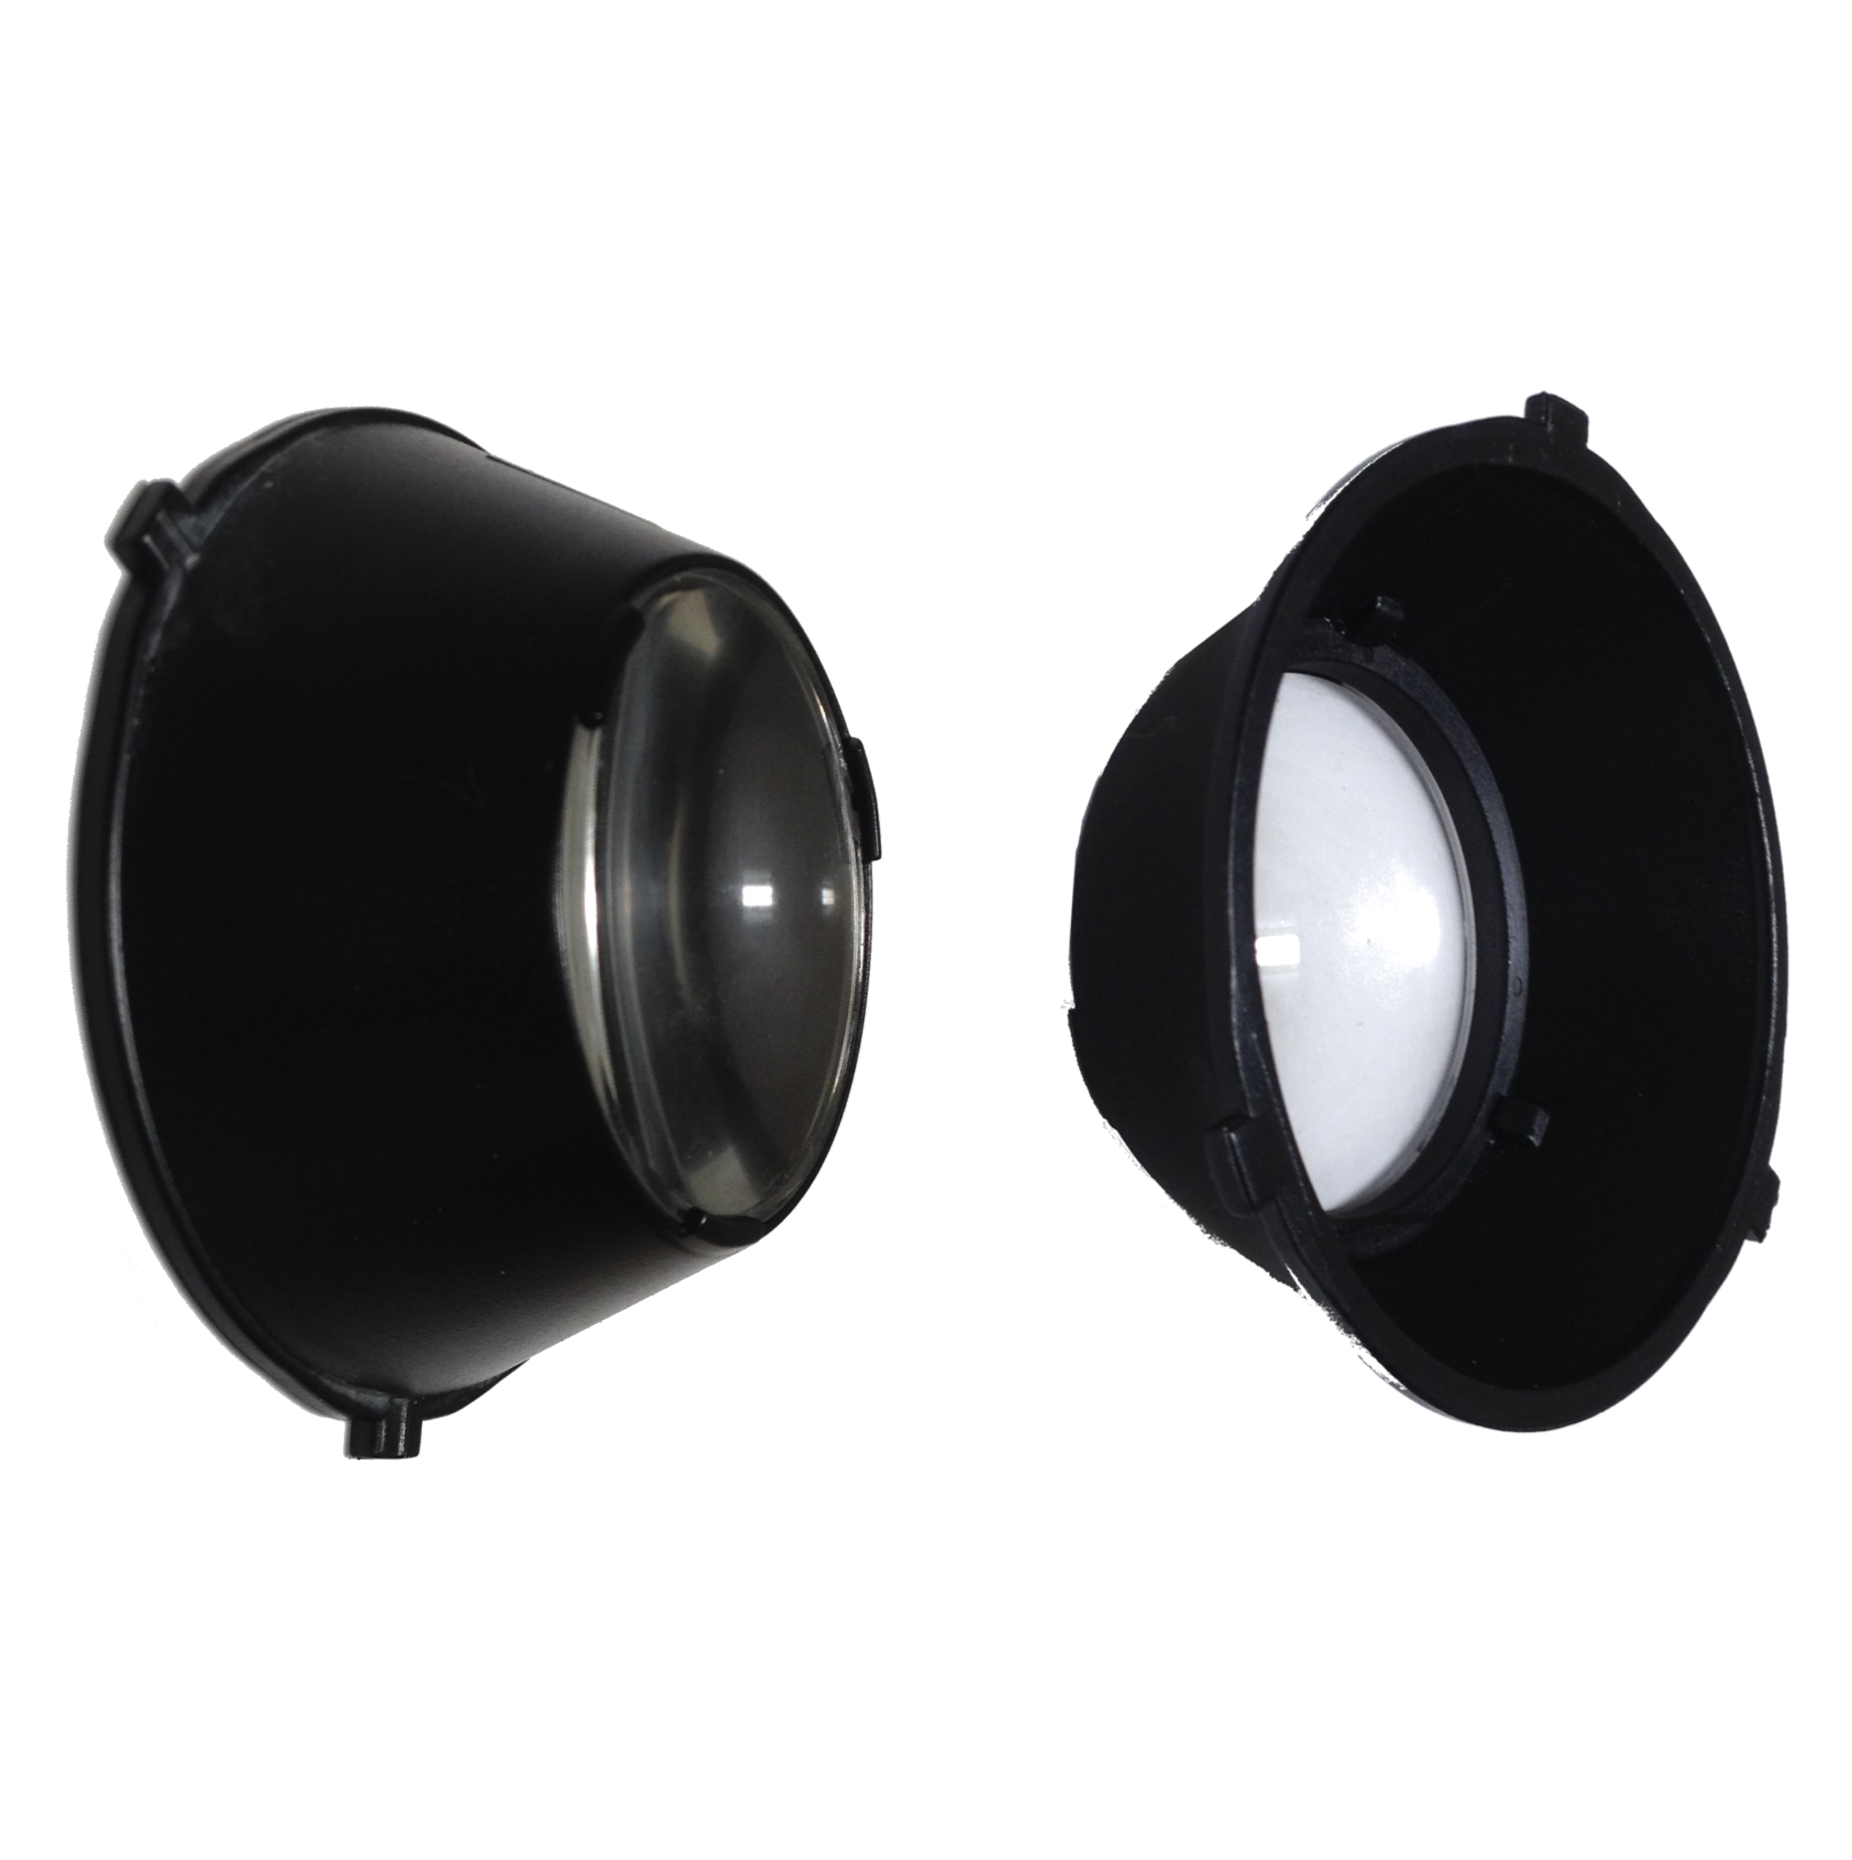
\includegraphics[width=0.5\linewidth]{resources/rift_lenses}
    \caption{Rift lens, front and back views}
	\label{fig:rift_lens}
\end{subfigure}    
    \caption{Comparison of lens complexity.}
    \label{fig:lens_comparison}
\end{figure}

\subsection{Using software to correct for distortions}
By comparison with an optical distortion correction system, software offers the attractive property of requiring no additional physical components, and so no additional hardware cost\footnote{Experience working for a consumer electronics company strongly suggests to me that this exact argument was used.}. A remarkable property of barrel and pincushion distortions is that the geometric shape has been distorted but \textit{the image is still in perfect focus}. This means that the distortion can be corrected for by moving pixel data around in the original image. The amount of movement required is a function of the radial distance from the optic axis \cite{Brunelli2009}. The barrel distortion in Figure \ref{fig:appearance_unprocessed} could be corrected by re-arranging pixel data, moving each pixel towards the centre of the lens to achieve the result shown in Figure \ref{fig:appearance_processed}.

The image processing required for this geometric correction can be done pixel-by-pixel. Given the size of the rift display, it must be computed for $1280 \times 800 = 1,024,000$ times per frame. If content is to be rendered at \SI{60}{Hz} then the total render time, of which the distortion step is only part, needs to take place in less than \SI{16}{ms}. Fortunately, the individual pixel calculations are entirely independent of one another, making the operation perfectly suited to parallel processing on a graphics card. 


\begin{figure}[htbp!]
\centering
\begin{subfigure}{0.8\textwidth}
    \centering
    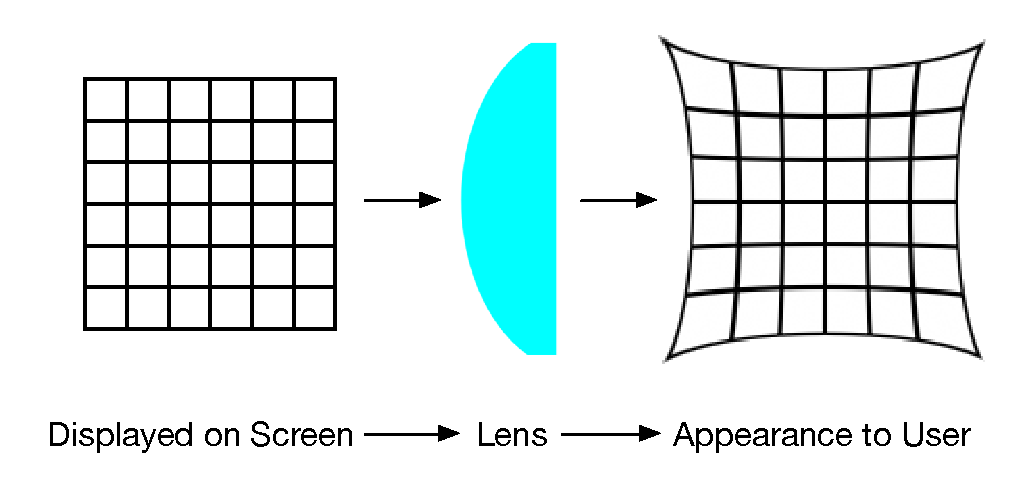
\includegraphics[width=0.8\linewidth]{resources/appearance_unprocessed}
    \caption{The appearance of native content to the Rift's user.}
	\label{fig:appearance_unprocessed}
\end{subfigure}
\centering
\begin{subfigure}{0.8\textwidth}
    \centering
    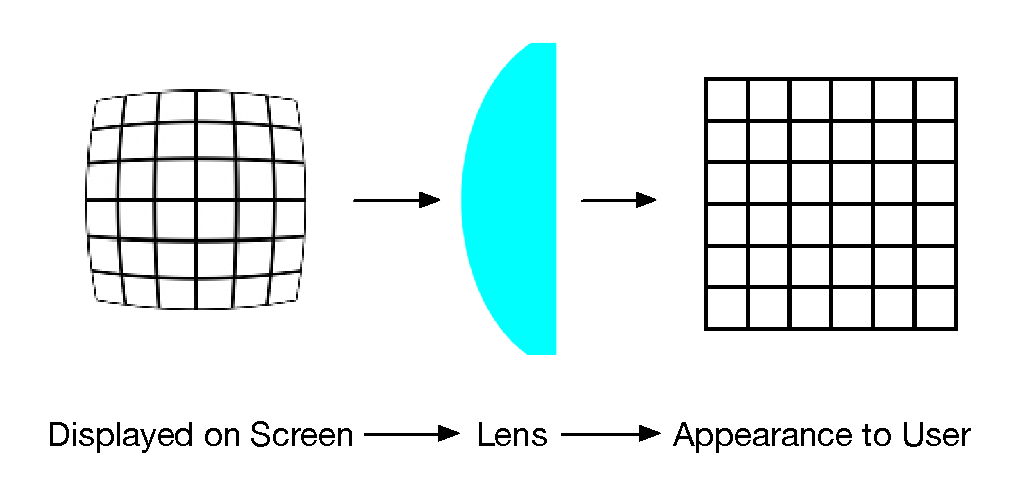
\includegraphics[width=0.8\linewidth]{resources/appearance_processed}
    \caption{The appearance of processed content to the Rift's user.}
	\label{fig:appearance_processed}
\end{subfigure}    
    \caption{Correcting distortion by modifying image content.}
    \label{fig:processing_content}
\end{figure}

\subsection{Using shaders to correct for distortions}
Modern 3D computer graphics make heavy use of Graphical Processor Units (GPUs), processors designed especially for the parallel execution of thousands or millions of independent calculations on pixel data. The image deformation problem is perfectly suited to be solved with a GPU. 

Two companies dominate the market for graphics cards: Nvidia and ATI. Graphics drivers are notorious for driver problems \footnote{When discussing problems in the department, the first question was frequently "What graphics card are you using". Using a moderately powerful Nvidia card with the latest drivers was a pragmatic way to avoid exotic hardware issues.}. The project chose to use a NVidia GeForce GTX 480 graphics card on the basis that it would support the most recent version of OpenGL (4.4 at the time of writing). Nvidia provide good driver support, and have created the CUDA parallel computing platform in case it was necessary to use the graphics hardware directly for calculations.

Similar to the division of the graphics card market, two main application programming interfaces (APIs) exist to make use of graphics hardware. These are Direct3D and OpenGL. The project chose to use OpenGL as it had previously been used in the MSC Graphics lectures, it is an open standard, and it is cross platform. By contrast, Direct3D appeared to be unfamiliar and would lock the project to the Windows operating system.

Once the pragmatic decisions regarding the choice of hardware and API were made, the practical work could begin: designing and implementing a graphics shader program to perform pixel-wise calculations.

\section{Designing a Test Shader}
Graphics shaders are executed on graphics hardware, not on the CPU. OpenGL shaders are written in the Graphics Library Shader Language (GLSL), a C-like language with the occasional surprise. They are massively parallel and difficult to debug, though some third party debugging tools do exist \cite{glslDevil}. There are no ways to print statements in GLSL \footnote{And in any case, if a per-pixel shader script is executed over a million times per frame, and at sixty frames per second, then print statements would not be a practical debugging tool}. For these reasons, the chosen approach for shader development was to start with a very simple shader, and gradually add complexity in a series of iterative steps. 

\subsection{Vertex and Fragment Shaders}
In a graphics pipeline there are vertex shaders and fragment shaders \footnote{Geometry shaders were added in OpenGL3.2 and and tessellation shaders added in OpenGL4, but these shaders are mainly intended to do geometric mesh adjustments and aren't relevant to the processing pipeline in this project.}. Vertex shaders are executed at every vertex in a scene, approximately thirty two thousand vertices in the case of the cortical surface content. Fragment shaders are executed at every fragment, the projection of an area of an object polygon onto a pixel in the screen. The final value of one screen pixel may be the combination of values of a number of fragments, combined as a function of their depth, opacity and position.

\subsection{Simple test shader design}
Listing \ref{simple_vert} shows the most basic vertex shader, where vertices are simply passed through the pipeline. The graphics pipeline is a state machine, so the variables \texttt{gl\_ModelViewProjectionMatrix} and \texttt{gl\_Vertex} are automatically set by the system, and the result of the calculation \texttt{gl\_Position} is automatically passed on to the next part of the pipeline.

\lstinputlisting
  [label=simple_vert, caption=A Simple Vertex Shader]{code/my_first_shader.vs}

Listing \ref{simple_frag} is almost as simple as the example vertex shader. It sets the colour of every fragment to red. If this fragment shader works, every polygon in the rendered object should be bright red and the background should not be altered. This sort of shader may seem excessively simple, but lots of simple checks were necessary to confirm that basic OpenGL functionality was achievable before moving on to more complicated things.

\lstinputlisting
  [label=simple_frag, caption=A Simple Frament Shader]{code/my_first_shader.fs}

\subsection{Including and compiling shaders}

As might be expected from the C-like form of GLSL, shaders need to be compiled before they can be executed on the GPU. Martin Christian's libglsl library was used to manage shaders, though the library needed to be adjusted to allow compatibility with current OpenGL and GLSL. 

Three different methods for using GLSL shaders were tried during the project. 
\begin{itemize}
\item Shaders can be written a separate plain text file and given an extension that helps to explain their content. It is conventional to give a vertex shader a .vs extension, and a fragment shader a .fs extension\footnote{or sometimes a .ps extension for 'pixel shader', as used in the ORIA project}. The shader file can then be opened and loaded at runtime. This is convenient as it means that altering the shader does not require re-compilation of the main body of source code. It also means that errors in the shader code do not generate compile errors and may only appear at runtime. 
\item In a similar way to reading in a plain text file, the shader may be defined as a string inside the source code. This can be useful for testing purposes, when checking that the program does indeed have access to the shader source at runtime. It also cuts down the number of files in the project, though at the expense of clarity! As the shader code is in string format, it is still not checked by the debugger and so is equally liable to runtime problems as if it were a separate file.
\item A sophisticated\footnote{translation: terrifying} third option is to load a compiled shader program as a binary file. This approach means that no shader compilation is required, but it means that the shader is no longer human-readable. Given the simplicity of the shaders in this project, and the need to frequently adjust their contents, this optimisation was unnecessary.
\end{itemize}

All three approaches to the use of GLSL shaders were used during the project. In-line shader code was used during early stage testing, whilst the libglsl shader was being upgraded to work with GLSL 440. Some publicly available Rift deformation shaders were in binary format, and were tested but could not be subsequently modified. The preferred approach, for elegance and practicality, was to have fragment and vertex shader files and load these at run-time.


\section{Applying Shaders in VTK}

Using a basic test shader, the next step was to use it in the VTK image processing pipeline. A number of potential options presented themselves, and a number of challenges were encountered.

\subsection{Applying GLSL Shaders to Materials}
Investigation revealed that applying GLSL Shaders to VTK scenes via material properties is not feasible in current versions of VTK.

One drawback of large open source projects is that the most widely available documentation may be severely out of date. In this regard, VTK is a victim of it's own success. A lot of documentation \cite{Seip2005}, \cite{OBrien2009} suggests that the GLSL shaders can be encapsulated within XML and applied to a VTK object as a material. This is also the approach of the official documentation \cite{VTK_XML_shaders}, where "To Do" and "In progress" comments create the deceptive appearance that these features are cutting edge. \textbf{Do not be fooled!} This use of shaders is deprecated, and has not been possible in 'recent' VTK versions for some time. Due to the size of the project it can be difficult to find documentation for every feature of interest, and confirming VTK feature deprecation was to become a reoccurring problem during the project\footnote{If there is one thing harder than finding a needle in a haystack, it is finding a needle in a haystack when the needle was quietly removed back in 2008.}.

\subsection{Applying GLSL Shaders to Objects}
Having learned to ignore VTK shader documentation pre-dating 2008, certain tutorials it transpired that shaders can be applied directly to VTK objects. This option, though initially promising, contained critical flaws. 

Firstly, the approach meant that the project had to switch from Python to C++. VTK is developed in C++ and other languages are supported via wrapper code. The wrapping does not always expose the full functionality of the source code, and in this case the functionality of the Shader2 class was discovered to be only partially exposed in Python. Although it should be possible to edit the VTK source and coax the parser into generating more complete Python wrappers, even the VTK authors at Kitware admit that this process can be "a bloody pain" \cite{VTK_Wrapper_FAQ}. With this warning in mind, it was decided to use C++ in order to get full access to the VTK classes.

Secondly, the documentation on this approach was very scarce. Another VTK user had recently raised this on a the VTK mailing list \cite{vtk_shader_actor}, and with this expert assistance a working solution was found. Listing \ref{object_shader} shows a functional implementation which was contributed to Stack Overflow in order to help document the process \cite{SO_shader_actor}. Note that unlike the test shader in Listing \ref{simple_frag} this shader cannot have a \texttt{main()} function, since that would cause a name conflict with other parts of the VTK render process. 

\lstinputlisting
  [label=object_shader, caption=Applying a Shader to a VTK Object]{code/vtk_object_shader.cpp}

Figure \ref{fig:object_shader} shows the result of the working example: any fragment that represents part of the cone object gets coloured red. 

\begin{figure}[htbp!]
    \centering
    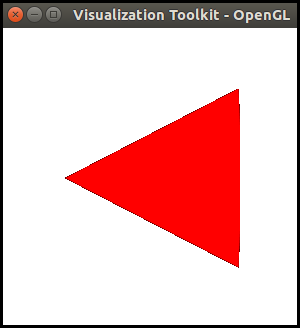
\includegraphics[width=0.5\textwidth]{resources/object_shader}
    \caption{A VTK object with GLSL shading.}
    \label{fig:object_shader}
\end{figure}

The third and most significant problem of the per-object shader approach can also be understood with reference to Figure \ref{fig:object_shader}. The target image deformation, as Figure \ref{fig:appearance_processed} showed earlier, is a barrel deformation. This means that pixel data must be radially displaced away from the optic axis. The cone shader does not, and cannot affect pixels beyond the surface of the cone, since the fragment shader is only executed for object object pixels, and default shaders are used to handle background pixels.  

These problems, in particular the third problem, led to the conclusion that object-shaders would not provide a viable method for performing image distortion suitable for Rift display.

\subsection{Applying GLSL Shaders to Buffers}
Given the requirement to apply a deformation across an entire screen, the the VTK multipass-rendering framework looked to be a good place to start. This framework allows users to specify custom rendering passes to a vtk renderer. Even better, Dr Bernhard Kainz, one of the members of the Biomedical Image Analysis Group, had previously written a custom rendering pass that could apply saliency filtering to image data.

\begin{figure}[htbp!]
    \centering
    
\includegraphics[width=0.5\textwidth]{resources/placeholder}
    \caption{Flow diagram showing the multipass framework}
    \label{fig:multipass_rendering}
\end{figure}

Several problems were overcome as these classes were adapted to work in the desired fashion.

Firstly, the \texttt{vtkRenderer->SetPass()} method, central to the entire approach, was quietly deprecated in VTK 6.x. Once identified,  the decision was made to work VTK 5.10, on the basis that it was the latest, and best version of VTK to be released where the \texttt{SetPass} could be found.

Next, the \texttt{SaliencyPass} code made use of a \textbf{glsl} library to load, compile and run \textbf{GLSL} shaders. This library worked with GLSL \texttt{\#version 110} but was incompatible with recent versions of GLSL. Certain functions in OpenGL 4.4 required GLSL \texttt{\#version 440} compatibility, and this in turn required that the glsl shader management class be updated. Fortunately, many of the deprecated functions had been implemented in recent OpenGL versions, and so many of the previously "experimental" ARB-functions could simply be replaced by modern "core" functions.

\begin{figure}[htbp!]
    \centering
    
\includegraphics[width=0.5\textwidth]{resources/placeholder}
    \caption{CPU and GPU domains, and methods of communication.}
    \label{fig:cpu_gpu_domains}
\end{figure}

Once the derived class could compile, a number of OpenGL problems needed to be solved. OpenGL appears to follow the "Silence is golden" design philosophy \cite{the_art_of_unix_programming}, and a programmer query OpenGL state to discover GLErrors. In the absence of diligent checks, these errors otherwise manifest themselves in terms of a blank render screen or segmentation fault at runtime. 

\lstinputlisting
  [label=gl_check_error, caption=Checking OpenGL error state]{code/gl_check_error.cpp}

Listing \ref{gl_check_error} shows how a simple helper function can be used to report error state. In order to pinpoint problems, the GL error state should be checked every time a non-trivial gl function call is made.



%Implementing OpenGL
%Fun with Uniforms
%Viewport Sizes
%Fun with transformation matrices
%Matrix stacks, pushing and popping
%FBOs, RBOs and textures (oh my!)
%Do you suffer from premature optimisation?



derived shader class could be built. Modifications to the derived class involved working with OpenGL functionality,  Development got a little more difficult as the 




In order to achieve the desired shader deformation, two different approaches need to be combined. Default rendering passes need to be defined explicitly and combined into a Sequence Pass, and then a new rendering pass needs to be derived to perform the desire deformation to the entire render scene at once. The full system is represented in Figure~\ref{fig:vtk_extended_pipeline}.

\begin{figure}[htbp!]
    \centering
    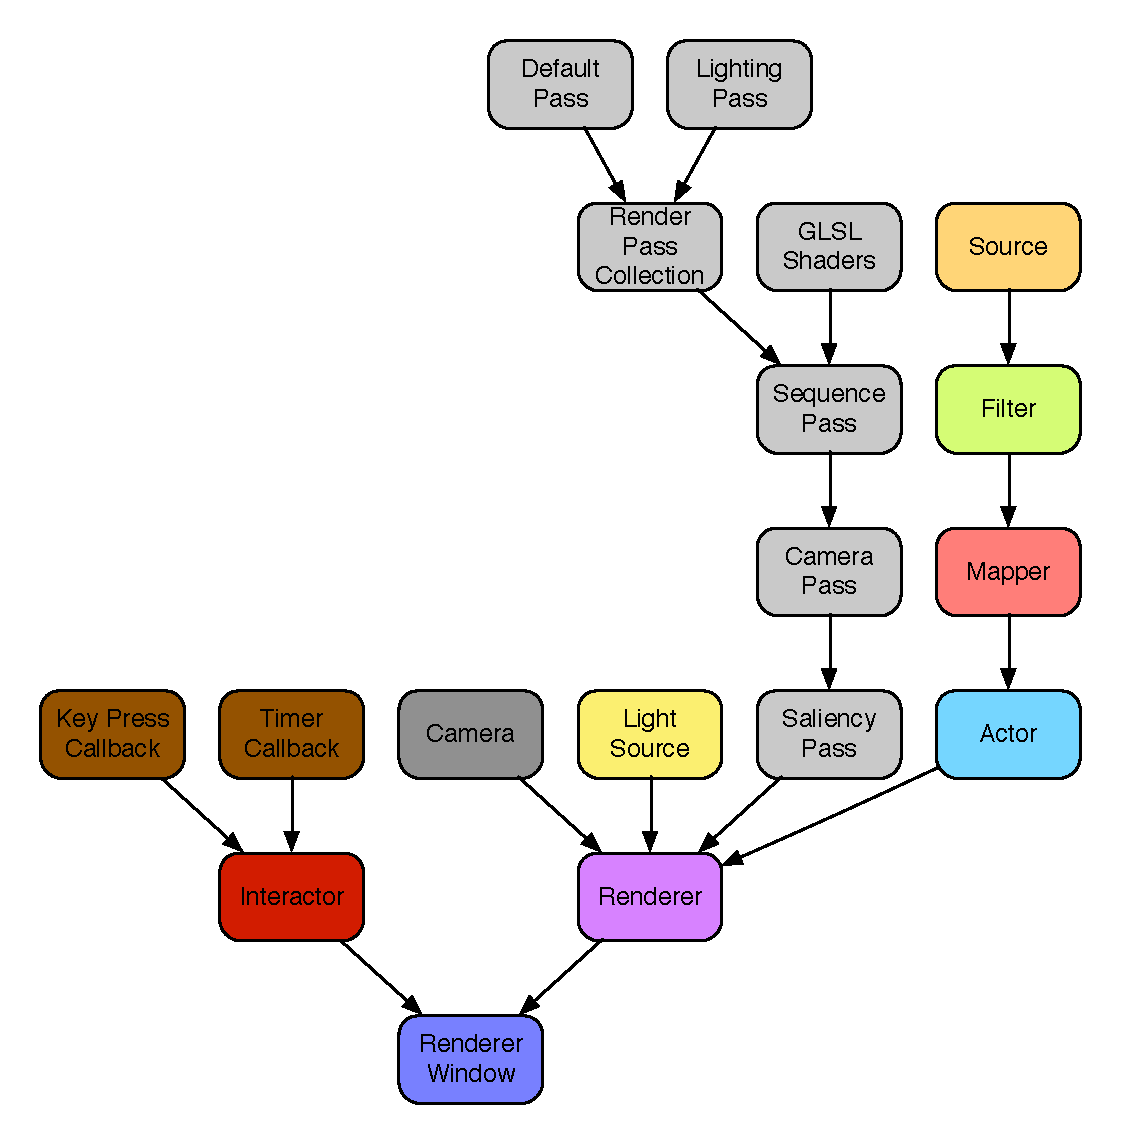
\includegraphics[width=1\textwidth]{resources/vtk_extended_pipeline}
    \caption{The Extended VTK Pipeline}
    \label{fig:vtk_extended_pipeline}
\end{figure}

Specifying the default rendering passes is necessary as VTK stops automatically defining them once the user manually configure any aspect of rendering. As shown in Figure~\ref{fig:vtk_extended_pipeline}, the default pass initializes the colour and depth buffers of the scene and the lighting pass sets up the scene lighting. VTK needs to apply these passes sequentially, and so they are grouped as a collection and then packaged into a Sequence Pass. The camera pass is applied after that sequence, and then the custom-made Saliency pass is applied. This is the point at which things start to get interesting.

The Saliency pass is derived from previous work by Dr Bernhard Kainz, and uses raw OpenGL code to perform off-screen rendering to a texture. This process, in effect, means that the scene is rendered to an area of memory on the graphics card instead of to pixels on the screen. The texture memory can be accessed very quickly by OpenGL functions, and is perfectly positioned for subsequent GLSL renderers.

\begin{figure}[htbp!]
    \centering
    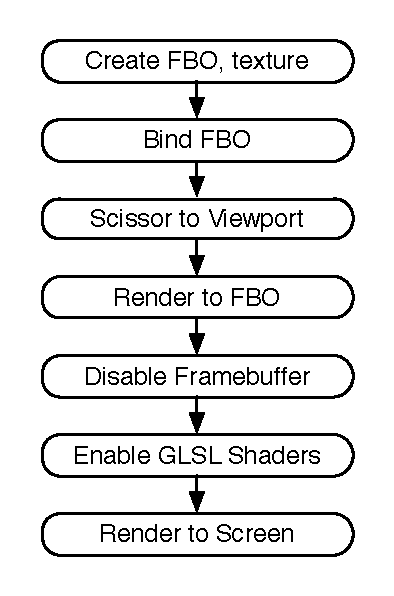
\includegraphics[width=0.4\textwidth]{resources/vtk_saliency}
    \caption{The New VTK Saliency Pass}
    \label{fig:vtk_saliency}
\end{figure}

TODO: This high-level description neatly side-steps the various issues of loading shaders, upgrading from glARB classes to modern glCore functions, ensuring that GLSL 440 was supported, upgrading the drivers, and the operating system, in order to get sufficiently recent NVIDIA support, and then dealing with the OpenGL bugs that recent versions of the NVIDIA drivers contain!! Though none of that was 'news-worthy', it took a great deal of time and patience to identify and fix. 

\section{Rift Deformation Shaders}
GLSL shaders are (ab)used to perform three functions in this project. They shift the image in order to align the camera viewpoint centre with the lens centre. They apply a barrel deformation of the entire image in order to compensate for the pincushion deformation of the Rift's lenses.  They also mask the edges of the screen where the OpenGL 340.x drivers leave image artefacts. 

\todo{discuss chroma issues}

It is assumed that the reader is familiar with the nature of shaders, and so the discussion here will not introduce the concept but rather will focus on the unusual way in which they are being employed. 

Figure~\ref{fig:rift_screen} shows how the lens positions, aligned with the user's eyes, are not aligned with the centre of the screen. This presents a problem, as the VTK cameras produce a viepoint that does not align with the user's eyes. The fragment shader code is executed for every pixel in the screen. Focussing first on the left-eye image, every fragment shader position is laterally offset by the lens centre to screen centre displacement. For the rift DK1 this involves a y-adjustment of 48 pixels. So when the shader is called for a pixel at (0, 0) the offset is applied and all subsequent calculations are made for a pixel at (48, 0). This is somewhat of a brute force solution, and will require revision for new hardware with different screen offsets. But given the hardware differences between the DK1 and DK2, it is likely that the shader code would need to be completely re-written.

\begin{figure}[htbp!]
    \centering
    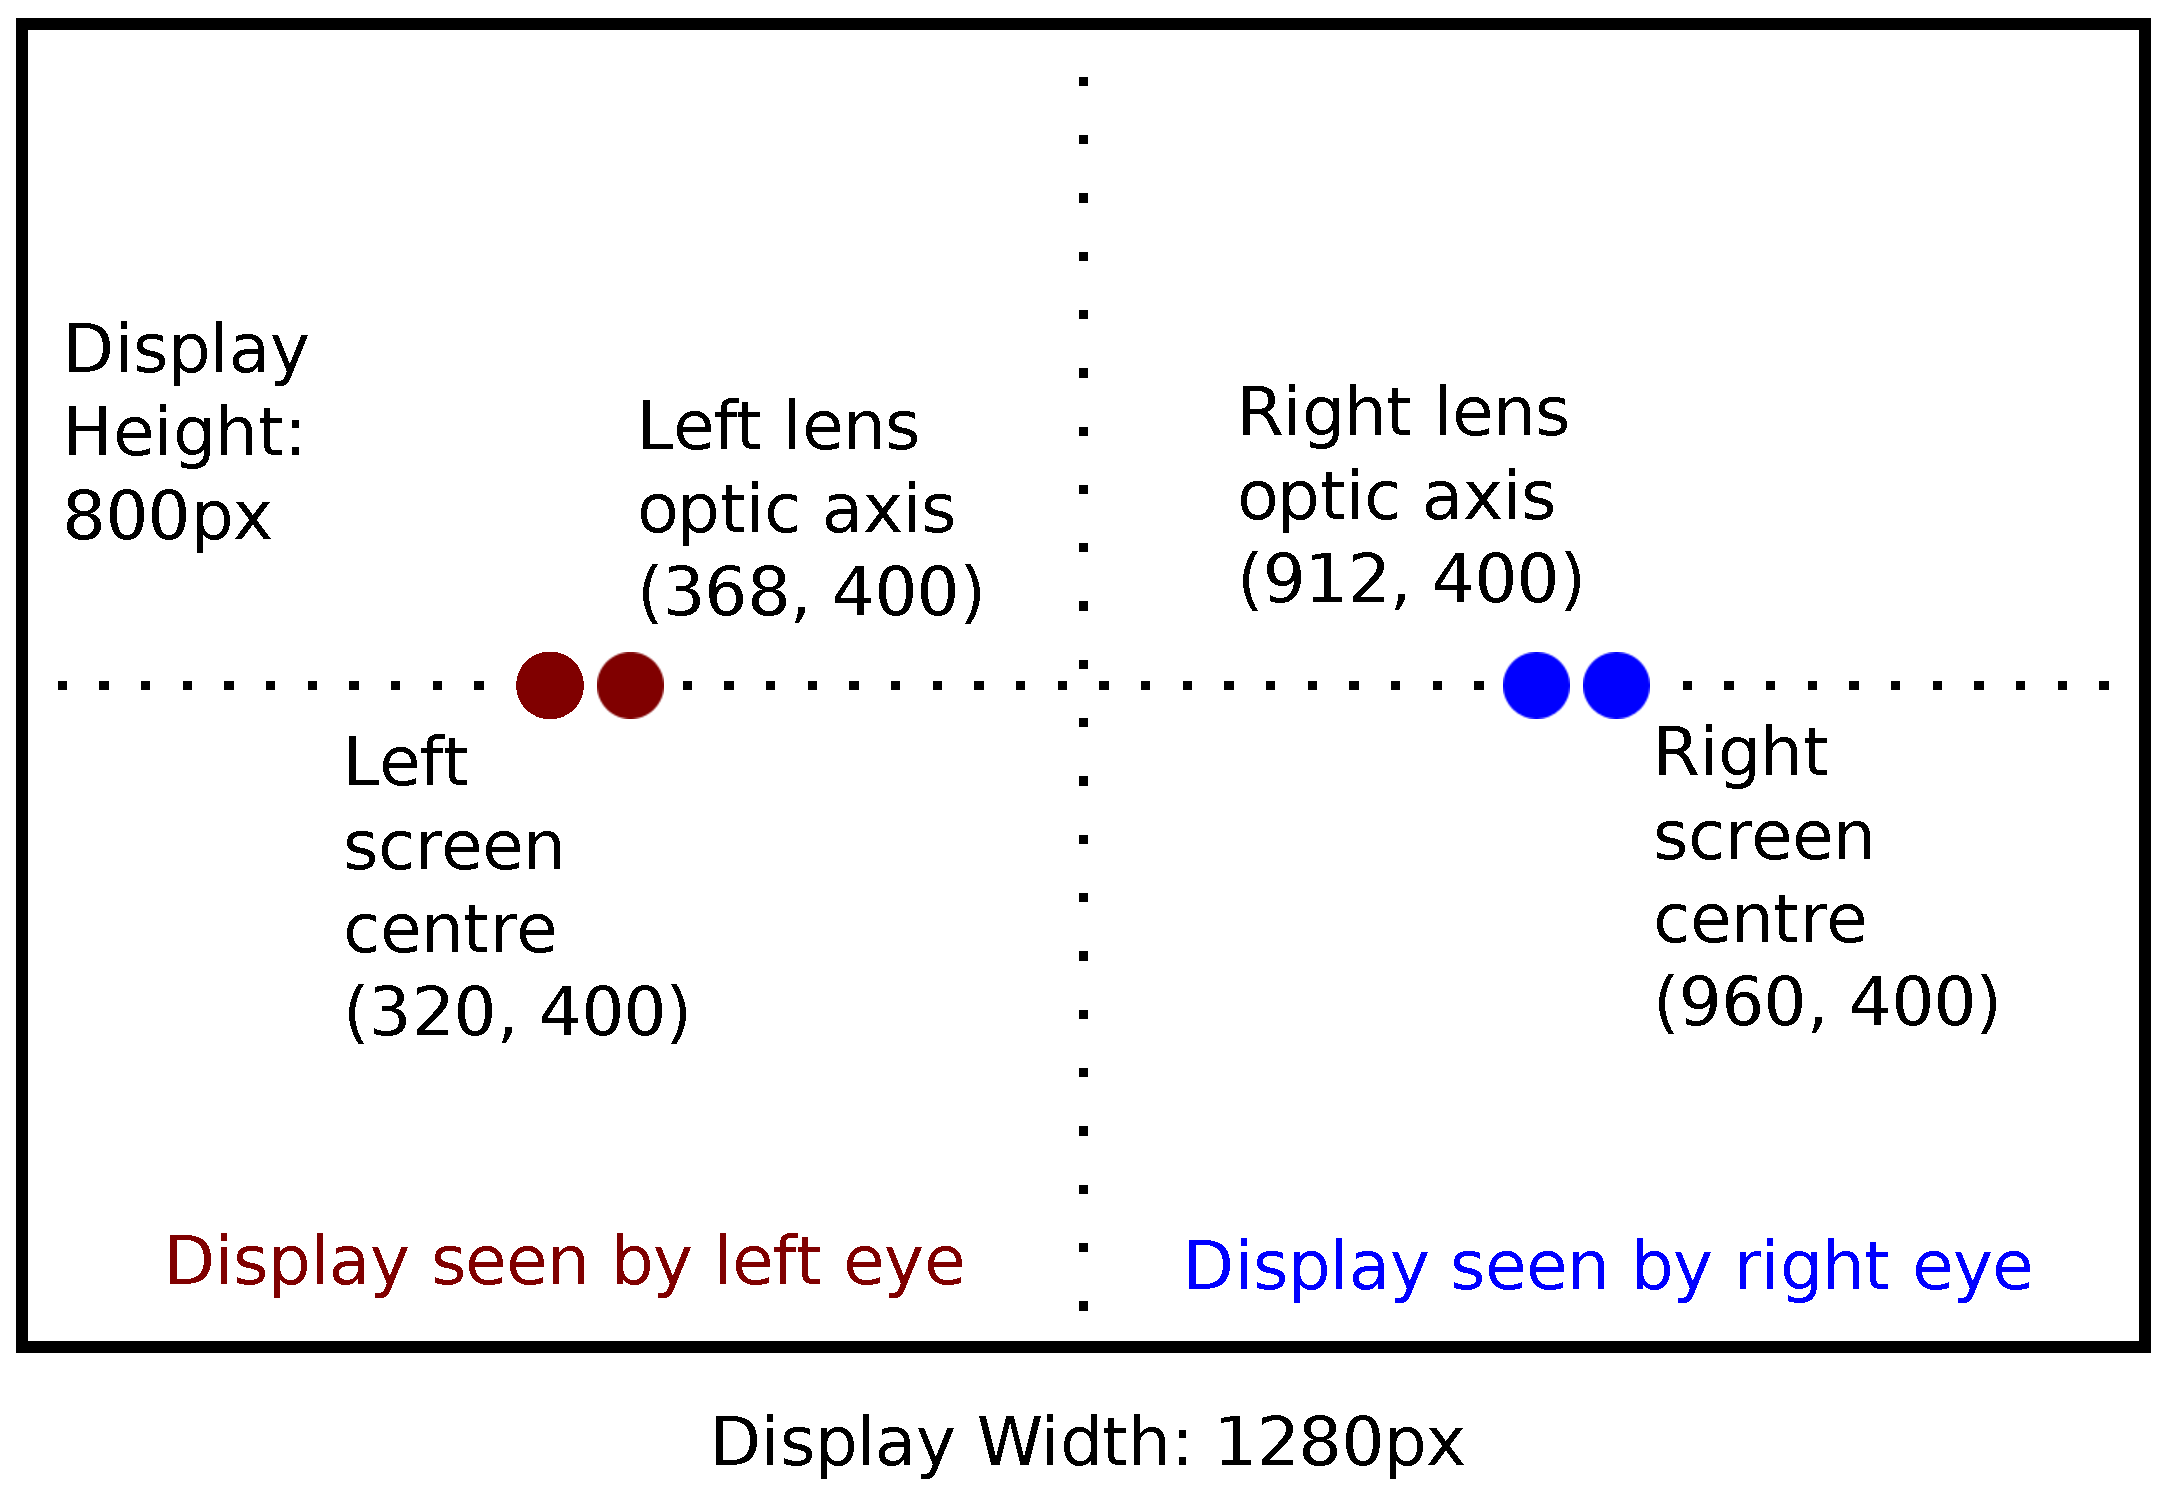
\includegraphics[width=0.8\textwidth]{resources/rift_screen}
    \caption{Lens and Screen Centres on the Rift Display}
    \label{fig:rift_screen}
\end{figure}

After correcting for the lens centre displacement, the shader then needs to pre-emptively correct for the pincushion distortion of the Rift lenses. This is achieved using a polynomial function of the pixel's radial displacement from the lens centre. The polynomial function is based on reverse engineering of the Rift SDK TODO: cite shader forum, and with parameters obtained from Dr Stephan Rogge TODO: another citation. 

TODO: Ask Daniel if there should be some maths in here. It all seems a little bland!

\begin{figure}[htbp!]
    \centering
    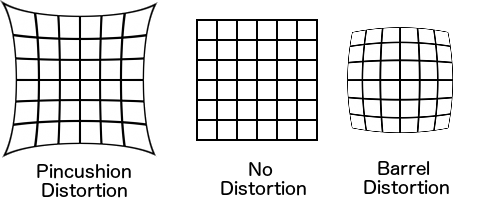
\includegraphics[width=0.8\textwidth]{resources/distortions}
    \caption{Lens distortions illustrated using a square grid.}
    \label{fig:distortions}
\end{figure}

After correcting for the lens distortion, it is desirable to apply a chromatic aberration factor in order to mitigate the dispersive effect of the Rift's lenses as mentioned in Section~\ref{sec:need_for_shaders}. The parameters for the chromatic aberration correction were not available, and so approximate parameters were chosen based on empirical testing. TODO: give this a go. 

\section{Practical notes}

\lstinputlisting
  [label=distortion_debugging, caption=Useful Code for Debugging Fragment Shaders]
  {code/Debugging.fs}
  
I *want* to complain here about how frustrating some of the driver problems were. Particularly the bug in NVIDIA 331.32 that "could prevent OpenGL Framebuffer Objects (FBOs) from being properly redrawn after a modeswitch.". Yes, NVIDIA, that bug certainly could! It took a long time to confirm that the problem was not due to my FBO rendering process, but rather due to driver problems.


\section{Other Approaches}
In theory, the Rift SDK can apply deformations directly, and since v0.3 Oculus have stated the SDK-rendering is the preferred approach. All of the example code for SDK-rendering was for a Windows system with DirectX rather than OpenGL, and it was decided that directly using GLSL shaders would be a more feasible approach given the project time frame. 

\chapter{Results}
The results section can talk about specifications of the final system, and the outcomes of the survey. This is looking quite promising. In particular, several people have had some interesting suggestions for future work. 

\section{Final System Specification}
The VR system developed in this project consists of two parts: a methodology for converting HCP data to a suitable form for importing into the VTK pipeline, and software that can load the generated data and render it to the rift display. 

The latter software consists of a C++ project requiring CMake, CTest, VTK5.10, GLEW and OpenGL. In addition, using the Rift requires linking with the GL, GLU, pthread, udev, rt, ncurses and X-Windows management libraries (Xinerama, Xrandr, Xxf86vm, Xi, X11) libraries. The project directory structure is shown in Figure \ref{fig:project_directory_structure}. Although currently running on Linux, the project has been kept as small and neat as possible in order to assist future development work. The dependencies listed are specific to Linux, but small modifications will allow it to run on MacOS\footnote{Mainly the removal of rt timer dependency, which is only used for latency measurements.}. Porting the project to Windows should also be fairly straightforward, and the project has already been run on a Windows system to when debugging Nvdia driver problems.

\begin{figure}
\centering
\framebox[\textwidth]{%
\begin{minipage}{0.9\textwidth}
	\dirtree{%
	.1 vtkRift/.
 	.2 CmakeLists.txt.
	.2 CTestCofig.cmake.
	.2 .git.
	.2 .gitignore.
	.2 build/. 
	.3 \ldots all built code. 
	.2 cmake/.
	.3 FindGLEW.cmake.
	%.2 documents/.
	%.3 rendertimes.xlsx.
	%.3 README.txt. % TODO
	.2 resources/.
	%.3 btain.vtk.
	.3 CCTracts.vtk.
	.3 FullBrain.vtk.
	.3 FullBrain2.vtk.
	.3 simple.fs.
	.3 simple.vs.
	.3 Distortion.fs.
	.3 Distortion.vs.
	.2 src/.
	.3 CmakeLists.txt.
	%.3 brain.cpp.
	%.3 cone.cpp.
	%.3 cone\_interactor.cpp.
	.3 main.cpp.             % TODO: rename multipass_vtk.cpp.
	.3 vtkRiftRenderPass.cpp. % TODO: rename vtk_SaliencyPass.cpp.
	.3 vtkRiftRenderPass.h.   % TODO: rename vtkSaliencyPass.h.
	.3 OculusSDK.
	.4 \ldots library files from SDK 0.3.2.
	.3 fbo.
	.4 \ldots fbo management library from Lefohn et al..
	%.4 framebufferObject.cpp.
	%.4 glErrorUtil.cpp.
	%.4 renderbuffer.cpp.
	%.4 framebufferObject.h.
	%.4 glErrorUtil.h.
	%.4 renderbuffer.h.
	.3 glsl.
	.4 \ldots libglsl from Christen, modified for OpenGL 4.4 compatibility.
	%.4 glinfo.cpp.
	%.4 glsl.cpp.
	%.4 glutils.cpp.
	%.4 textureInfo.h.
	%.4 glinfo.h.
	%.4 glsl.h.
	%.4 glutils.h.
	.3 riftclass.
	.4 riftclass.h.
	.4 riftclass.cxx.
	}
\end{minipage}
}
\caption{Project directory content and structure}
\label{fig:project_directory_structure}
\end{figure}



\section{Objective Performance Metrics}

The most important metrics for the Rift display system are the resolution of the display, and the render speed of the image processing.

The resolution of the display is a little more complex an issue than it may at first appear. The Rift DK1 display is 1280 pixels wide, by 800 pixels high and each pixel is comprised of red, green and blue subpixels in an RGB stripe format\footnote{The DK2 uses Samsung's proprietary PenTile pixel layout, which complicates the issue of effective resolution even further}. The screen is \SI{149.76}{cm} by \SI{93.6}{cm} in size\footnote{or \SI{7}{inches} diagnonal} meaning that the pixel size is \SI{117}{\um} square. The results in a resolution of \SI{217}{pixels per inch}\footnote{Again, display dimensions are measured in inches. It is a strange industry.}



Quantifying display technology performance of high-quality displays is notoriously difficult and leads to the development of remarkable metrics such as "Just noticeable difference"\cite{Zhang2008} \footnote{Or manufacturing claims about "Retina" displays...}. The most important objective there are often easily quantifiable metrics to measure, in this case the render time and display resolution.

Early testing involved a Brain Surface object created from  


\begin{figure}[htbp!]
    \centering
    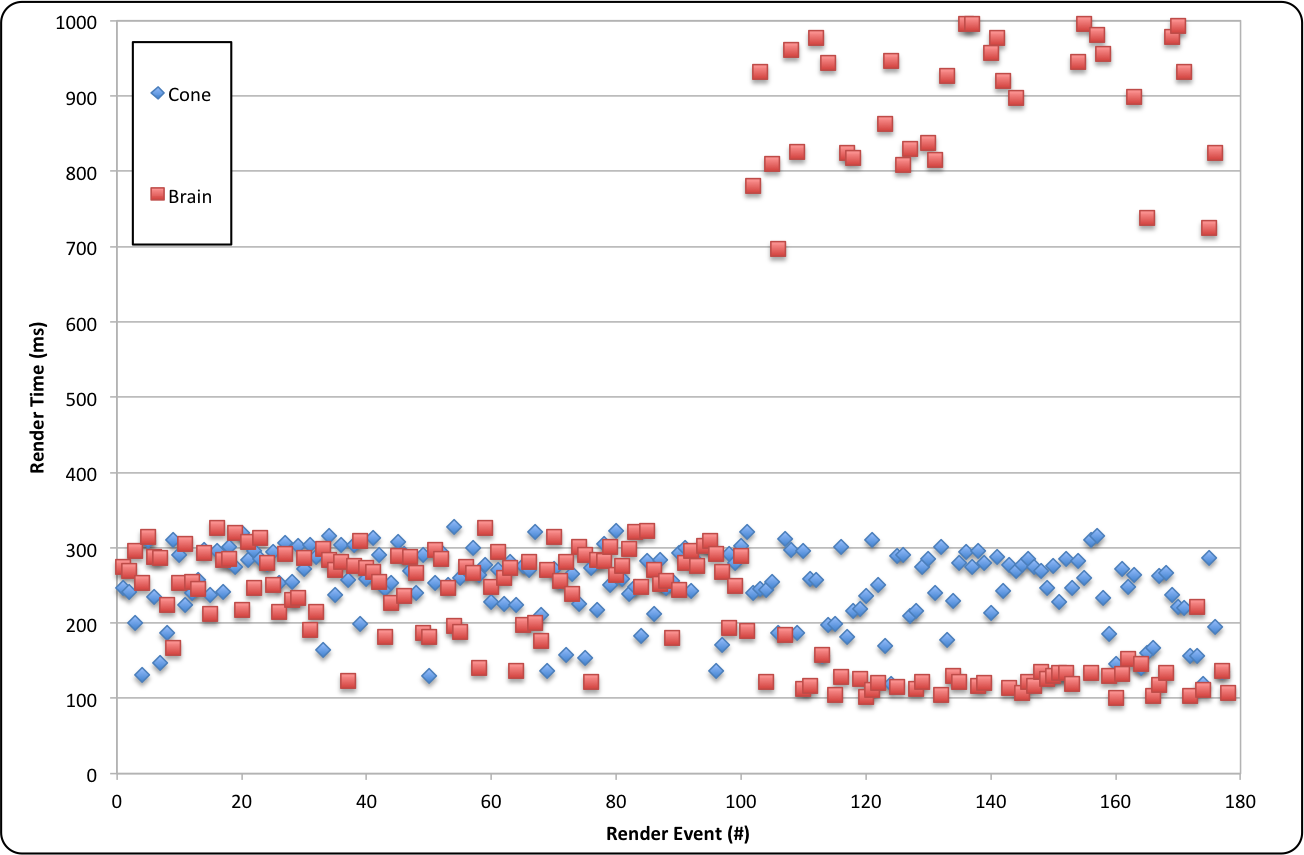
\includegraphics[width=0.8\textwidth]{resources/render_times}
    \caption{Times to render a primitive and \SI{100}{\mega\byte} Connectome Mesh.}
    \label{fig:render_times}
\end{figure}


\section{User Survey of the Biomedical Image Analysis Group}



\section{Automated Testing with CTest and CDash}
Early in the project, the decision was made to postpone testing until the structure of the application was known. The project was frequently required to adapt to new constraints\footnote{The operating system used for development changed twice times and the main programming language changed three times}, so this was approach was pragmatic though inelegant approach. Once the rendering system was capable of generating content, an automated testing system was implemented.

Of the non-imaging products developed by Kitware Inc, the most famous is probably CMake. This utility allows the automatic generation of configuration files like Makefiles and VisualStudio project files. It also allows automatic dependency management and smart configuration of common libraries and headers. A lesser known Kitware product is CDash, which works in conjunction with CMake to allow the automated testing, uploading of results and Dashboard display via a web-broswer. Listing \ref{configuring_ctest} shows the the simplicity of enabling CTest from within the project's top-level CMake file. Specific tests are configured as shown in Listing \ref{setting_a_test}, from the CMakeLists file containing the binary build settings.

\begin{lstlisting}[label=configuring_ctest, caption=Enabling CTest in the CMakeLists]
# Set up dashboard and testing
include(CTest)
enable_testing()
# CTestConfig.cmake is specific to the CDash web service
include(${CMAKE_CURRENT_SOURCE_DIR}/CTestConfig.cmake)
\end{lstlisting}

\begin{lstlisting}[label=setting_a_test, caption=Configuring a specific test]
# Add test format(test_name executable_name)
add_test( test_cone cone )
\end{lstlisting}

Using CDash for a project of this size is, admittedly, overkill. The product is designed to be used with large, complex projects where small changes can cause unexpected and subtle bugs unless automated testing is used. The argument in favour of using CDash was the elegance of automatic testing, and given that CDash was the only Kitware platform that \textit{wasn't} already used in the project\footnote{Paraview was used to view tractographies during content conversion, and ITK was used indirectly by ITK-SNAP.}, it needed to be used to complete the set!

CTest allows the creation of automatic test scripts that can be configured to run with command line parameters and options. These test scripts can be set to run at a pre-determined day, and can upload a log of test results to a remote server. For convenience, the kitware's free CDash server was used to receive and display the result of the testing. The results of one day's testing is shown in Figure \ref{fig:cdash_testing}. 

\begin{figure}[htbp!]
    \centering
    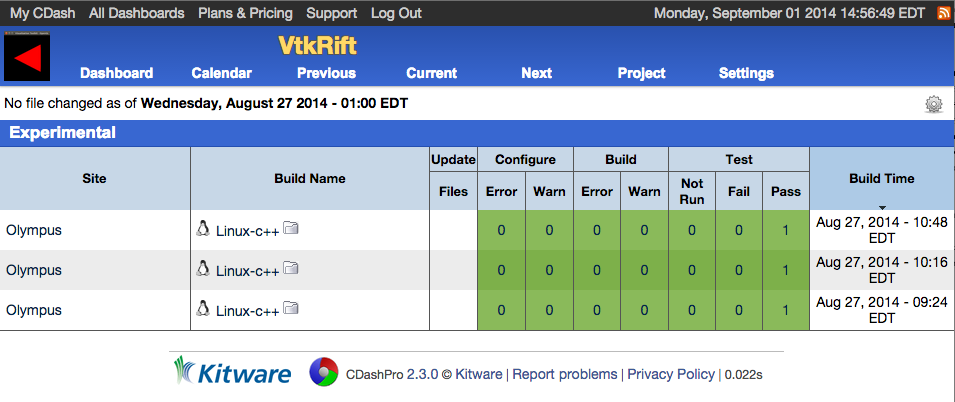
\includegraphics[width=0.9\textwidth]{resources/cdash_testing}
    \caption{Daily testing results via the CDash web interface.}
    \label{fig:cdash_testing}
\end{figure}

\chapter{Conclusion}
The project fulfilled it's goal of providing a full content conversion and rendering pipeline for medical image content. A number of significant technical challenges were encountered, but with the support of experienced computer graphics and medical imaging experts all of these were overcome. The final implementation could generate cortical surface or tractography models from a Human Connectome Project dataset and display these models in a 3D virtual reality environment. 

Survey participants evaluating the virtual reality system showed a strong interest in the interactive and 3D nature of the content, although they also highlighted numerous practical problems of the current system. Many of the practical problems reported by users may be solvable with further development: issues of tracking latency and image quality may already be fixed in the newly released Oculus Rift DK2. Issues of representing and interacting with image data have been discussed, and further work suggested. The demonstration system should serve as a useful starting point for any future development.

The success of this project will ultimately be measured in terms of its impact on other people. Demonstrations thus far have been well received, and the quality of insightful feedback shows that there are . It is hoped that the project has been a useful example of how state-of-the-art consumer VR technology can be applied, and that it will help to foster further ideas and developments. 
 

\bibliography{bibtex/connectome}	
\bibliographystyle{unsrt} % unsrt == order of appearance, != alphabetical

\appendix
\chapter{User Experience Survey}

\noindent \textit{Users completed a Google Form survey, and responses were automatically collated into a spreadsheet. An ellipsis is used here to indicate where participants provided verbal answers. Questions, suggestions and constructive criticism arising during the demonstratino were also recorded.}

\section*{1 Introductory Questions}

\Qitem{ \Qq{Name}: \hskip0.5cm\ldots }

\Qitem{ \Qq{Status:} 
\vskip0.1cm 
\QO{} MSc Student
\hskip0.5cm 
\QO{} PhD Student 
\hskip0.5cm 
\QO{} PostDoc
\hskip0.5cm 
\QO{} Other}

\Qitem{ \Qq{Commonly used medical imaging software:} 
\vskip0cm \QO{} VTK			\Qtab{4cm}{ \QO{} XMedcon }
\vskip0cm \QO{} ITK	 		\Qtab{4cm}{ \QO{} ImageJ }
\vskip0cm \QO{} IRTK			\Qtab{4cm}{ \QO{} Amide }
\vskip0cm \QO{} ITK-SNAP		\Qtab{4cm}{ \QO{} 3D Slicer }
\vskip0cm \QO{} MITK			\Qtab{4cm}{ \QO{} OSIRIX }
\vskip0cm \QO{} DTI-TK		\Qtab{4cm}{ \QO{} imagemagick }
\vskip0cm \QO{} Paraview		\Qtab{4cm}{ \QO{} SimpleDICOM }
\vskip0cm \QO{} RView		\Qtab{4cm}{ \QO{} Connectome Workbench }
\vskip0cm \QO{} Camino		\Qtab{4cm}{ \QO{} Other \hskip0.5cm\ldots }
}

\Qitem{ \Qq{Functionality desired in a visualisation tool:} 
\hskip0.5cm\ldots }
\clearpage

\section*{2 Demonstration Feedback}

\Qitem{ \Qq{Previous experience with VR Technology:} 
\vskip0.1cm \QO{} None 
\hskip0.5cm \QO{} A little 
\hskip0.5cm \QO{} A lot 
\hskip0.5cm \QO{} Developer
}

\Qitem{ \Qq{Immediate reaction to the VR demonstration:} 
\vskip0.1cm \QO{} Enthusiastic
\hskip0.5cm \QO{} Positive
\hskip0.5cm \QO{} Indifferent
\hskip0.5cm \QO{} Hated it
}

\Qitem{ \Qq{Viewing problems specific to the lenses:} 
\vskip0.1cm \QO{} None
\hskip0.5cm \QO{} Some
\hskip0.5cm \QO{} Significant
\hskip0.5cm \QO{} Intolerable
}

\Qitem{ \Qq{Can you see stereo 3D?} 
\vskip0.1cm \QO{} Yes. \hskip0.5cm \QO{} No.
}

\Qitem{ \Qq{Demo experience:} 
\vskip0.1cm \QO{} Fun and enjoyable
\vskip0.1cm \QO{} Fun, quickly became acclimatized
\vskip0.1cm \QO{} Initial disorientation but got used to it
\vskip0.1cm \QO{} Severe disorientation / nausea
}

\Qitem{ \Qq{Did anything specific trigger the disorientation?}
\hskip0.5cm\ldots }

\Qitem{ \Qq{How did you attempt to manage the disorientation?}
\hskip0.5cm\ldots }

\Qitem{ \Qq{Overall Experience} 
\vskip0.1cm horrible \Qrating{10} fantastic}
\clearpage

\section*{3 Technical Feedback}

\minisec{Please evaluate the following:}
\vskip.5em
\Qitem[a]{ \Qq{Latency} 
	\vskip0.1cm fine \Qrating{10} unusable}
\Qitem[b]{ \Qq{Screen resolution} 
	\vskip0.1cm fine \Qrating{10} unusable}
\Qitem[c]{ \Qq{Interaction tools} 
	\vskip0.1cm fine \Qrating{10} unusable}
\Qitem[d]{ \Qq{Stereoscopic depth} 
	\vskip0.1cm fine \Qrating{10} unusable}
\Qitem[e]{ \Qq{Image artefacts} 
	\vskip0.1cm fine \Qrating{10} unusable}


\Qitem{ \Qq{Preferred use type?} 
\vskip0.1cm \QO{} Monoscopic. \hskip0.5cm \QO{} Stereoscopic.
}

\Qitem{ \Qq{Would 'real world' cues be useful in the scene?} 
	\vskip0.1cm undesirable \Qrating{10} essential}

\Qitem{ \Qq{Other comments:}
\hskip0.5cm\ldots }

\chapter{Final Rift Shaders}

\lstinputlisting
  [label=distortion_vert, caption=The Vertex Distortion Shader]
  {code/Distortion.vs}
  

\lstinputlisting
  [label=distortion_frag, caption=The Frament Distortion Shader]
  {code/Distortion.fs}

\end{document}